% ----------------------------------------


\documentclass[a4paper,12pt]{article}

\usepackage{amsmath,amssymb,graphicx,amsthm,ifthen,epstopdf,fancyhdr,color}
\usepackage[margin=3cm,vmargin={2cm,3.5cm},includefoot]{geometry}
\usepackage[bookmarks=true]{hyperref}
\usepackage{booktabs}
\usepackage{palatino,rotating}
\usepackage{cite}
\usepackage{fancyhdr}
\pagestyle{fancy}

\fancyhf{}

\fancyhead[LO,RE]{\nouppercase{\leftmark}}
\fancyhead[RO,LE]{\textbf{\thepage}}
\renewcommand{\headrulewidth}{0.2pt}
\addtolength{\headheight}{50pt}

\newcommand{\TODO}[1]{ {\tt \color{red} [TODO:#1] } }
% Comment
\newcommand{\comm}[1]{ {\tt \color{blue} [Comment:#1] } }

\DeclareMathOperator{\tr}{tr}
\DeclareMathOperator{\Ev}{E}
\newcommand\x{\times}
% vector notation
\newcommand{\V}[1]{\ensuremath{\mathbf{#1}}}


% mathbb
\newcommand{\R}{\ensuremath{\mathbb{R}}}
\newcommand{\E}{\ensuremath{\mathbb{E}}}
\newcommand{\C}{\ensuremath{\mathbb{C}}}
\newcommand{\Fc}{\ensuremath{\mathcal{F}}}

\newcommand{\m}{m}

% simple norm
\newcommand{\norm}[1]{\left|\left| #1 \right|\right|}

\newcommand{\specstat}{\ensuremath{\Psi}}
\newcommand{\vx}{\ensuremath{\mathbf{x}}}
\newcommand{\Xk}{\ensuremath{X_K}}
\newcommand{\Xkn}{\ensuremath{X_{K_n}}}
\newcommand{\Gk}{\ensuremath{G_K}}
\newcommand{\Gkn}{\ensuremath{G_{K_n}}}
\newcommand{\Fkn}{\ensuremath{F_{K_n}}}


\begin{document}


\title{Random Subsets of Structured Deterministic Frames have MANOVA Spectra}


\author{
    Marina Haikin \footnotemark[1]
    \and 
    Ram Zamir \footnotemark[1]
    \and
    Matan Gavish \footnotemark[2]
}

\date{}
\maketitle

\renewcommand{\thefootnote}{\fnsymbol{footnote}}
\footnotetext[1]{EE - Systems Department, Tel Aviv University, Tel Aviv, Israel}
\footnotetext[2]{School of Computer Science and Engineering, Hebrew University of
Jerusalem}
\renewcommand{\thefootnote}{\arabic{footnote}}

\begin{abstract}
%   
We draw a random subset of $k$ rows from a frame with $n$ rows (vectors) and $m$
columns (dimensions), where $k$ and $m$ are proportional to $n$.  For a variety
of important deterministic equiangular tight frames (ETFs) and tight non-ETF
frames, we consider the distribution of singular values of the $k$-subset
matrix.  We observe that for large $n$ they can be precisely described by a
known probability distribution -- Wachter's MANOVA spectral distribution, a
phenomenon that was previously known only for two types of random frames.  In
terms of convergence to this limit, the $k$-subset matrix from all these frames
is shown to be empirically indistinguishable from the classical MANOVA (Jacobi) random matrix
ensemble.  
Thus empirically the MANOVA ensemble offers a universal description
of the spectra of randomly selected
$k$-subframes, even those taken from deterministic frames. The same
universality phenomena is
shown to hold for notable random frames as well.
This description enables exact calculations of properties of solutions for
systems of linear equations based on a random choice of $k$ frame vectors out of
$n$ possible vectors, and has a variety of implications for erasure coding,
compressed sensing, and sparse recovery.  
When the aspect ratio $m/n$ is small, the MANOVA spectrum tends to the well
known Mar\u cenko-Pastur distribution of the singular values of a Gaussian
matrix, in agreement with previous work on highly redundant frames.
Our results are empirical, but they
are exhaustive, precise and fully reproducible.
%
\end{abstract}

{\small
\noindent {\bf Keywords.}
Deterministic frames | 
equiangular tight frames |
MANOVA |
Jacobi ensemble |
restricted isometry property |
Gaussian channel with erasures |
Grassmannian frame |
Paley frame |
random Fourier |
Shannon transform |
analog source coding.
}
~\\


\noindent
Consider a frame $\{\vx_i\}_{i=1}^n \subset \R^\m$ or $\C^\m$ 
and stack the vectors as rows to obtain the $n$-by-$\m$ frame matrix $X$. 
Assume that $\norm{
\vx_i}_2=1$ (deterministic frames) or 
%The frame vectors have a unit norm (for random frames
$\lim_{n\to \infty}\|\vx_i\|=1$ almost surely (random frames). 
This paper studies properties of a random subframe 
$\{\vx_i\}_{i\in K}$, where $K$ is chosen uniformly at random 
from $[n]=\left\{ 1,\ldots,n \right\}$ and $|K|=k\leq n$.
%and
%$K\subset [n]$ for a subset with $|K|=k$,
We let $\Xk$ denote  
the $k$-by-$\m$ submatrix of $X$ created by picking only
the rows $\{\vx_i\}_{i\in K}$; call this object {\em a typical $k$-submatrix
of $X$}.
We consider 
%an interesting class of 
a collection of well-known 
deterministic frames, listed in Table \ref{frames:tab}, 
which we denote by $\cal X$. Most of the frames in $\cal
X$ are equiangular tight frames (ETFs), and some are near-ETFs.

This paper suggests that for a frame in $\cal X$ it is possible to calculate
%This paper suggests that for a variety of deterministic
%and random frames it is possible to calculate
quantities of the form $\E_K \specstat(\lambda(\Gk))$, 
where $\lambda(\Gk)=(\lambda_1(G_K),...,\lambda_k(G_K))$ is the
vector of eigenvalues of the $k$-by-$k$ Gram matrix $\Gk=\Xk \Xk'$
%\TODO{$\Xk\Xk'$ or $\Xk'\Xk$}
and $\specstat$ is a functional of these eigenvalues.
As discussed below, such quantities are of considerable interest in various
applications where frames are used, across a variety of domains, including
compressed sensing, sparse
recovery and erasure coding.

We present a simple and explicit formula for calculating 
$\E_K \specstat(\lambda(\Gk))$ for a given frame in $\cal X$ and a given spectral 
functional $\specstat$. Specifically, for the case $k \le m$,
\[
\E_K\specstat(\lambda(\Gk)) \approx \specstat\left( f^{MANOVA}_{\beta,\gamma}
\right)\,, \] 
where $\beta=k/\m$, $\gamma=\m/n$ and where 
$f^{MANOVA}_{\beta,\gamma}$ is the density of
Wachter's classical 
MANOVA$(\beta,\gamma)$
limiting distribution \cite{wachter}. The fluctuations about this approximate 
value are given {\em exactly} by
\begin{eqnarray} \label{main_for:eq}
\E_K \big| \specstat(\lambda(\Gk)) - \specstat\left( f^{MANOVA}_{\beta,\gamma}
\right)\big|^2 =   
C n^{-b} \log^{-a}(n) \,.
\end{eqnarray}
%\TODO{exponent of log is a or -a?}
While the constant $C$ may depend on the frame, 
the exponents $a$ and $b$ are {\em universal} and depend only 
on $\specstat$ and on the aspect ratios $\beta$ and $\gamma$. 
Evidently, the precision of the MANOVA-based approximation is good, known, and 
improves as $m$ and $k$ both grow proportionally to $n$.

Formula \ref{main_for:eq} is based on a far-reaching 
{\em universality hypothesis}: 
For all frames in $\cal X$, as well as for well-known random frames also listed in
Table \ref{frames:tab}, we find that
%For a large variety of frames in $\cal X$, we find that
the spectrum of the typical $k$-submatrix ensemble is indistinguishable 
from that of the classical MANOVA (Jacobi) random matrix ensemble
\cite{forrester}
of the same
size. 
(Interestingly, it will be shown that for deterministic ETFs this
indistinguishably holds in a stronger sense than for deterministic non-ETF
frames.)
%Interestingly, for equiangular tight frames (ETFs) this
%indistinguishably holds in a stronger sense than for non-ETF frames.
This universality is not asymptotic, and concerns 
finite $n$-by-$\m$ frames. However, it does imply that the spectrum of the
typical $k$-submatrix ensemble converges to 
a  universal limiting distribution, which is non other than 
Wachter's  
MANOVA$(\beta,\gamma)$ limiting distribution \cite{wachter}. 
It also implies that the universal exponents $a$ and $b$
in \eqref{main_for:eq}
are previously unknown, universal quantities corresponding to the 
classical MANOVA (Jacobi) random matrix ensemble.
%(ii) For the expected value of a spectral functional $\specstat$ over
%  the ensemble of typical $k$-submatrices of an $n$-by-$m$ frame matrix 
%  $X$, the above implies  
%  \[
%    \E_K\specstat(\lambda(\Gk)) = \specstat\left( f^{MANOVA}_{\beta,\gamma}
%  \right)\,. \] 
%  But in fact a stronger universality holds, namely
%  \[
%    \E_K \big| \specstat(\lambda(\Gk)) - \specstat\left( f^{MANOVA}_{\beta,\gamma}
%    \right)\big|^2 =   
%    C n^{-b} \log^a(n) \,.
%  \]
%  While the constant $C$ may depend on the frame, 
%  the exponents $a$ and $b$ are universal and depend only 
%  on $\specstat$ and on $n,m,k$. 

%In short, our conjectures imply that, as a random matrix ensemble,
%the typical $k$-submatrix of various frames is indistinguishable
%from classical MANOVA (Jacobi) random matrix ensemble, and for ETFs this
%indistinguishably is in a strong sense.  
%As a result, it is possible to calculate $\E_K\specstat(\lambda(\Gk))$ for
%specific frames and specific values of $\m,n$ and $k$ to known and good 
%precision. 

%These calculations are
This brief announcement tests Formula
\ref{main_for:eq} and the underlying universality hypothesis
by conducting substantial computer
experiments, in which a large number of random $k$-submatrices are generated. 
%
We  study a large variety of  deterministic frames, both
real and complex. In addition to the universal object (the MANOVA ensemble)
itself, 
we study difference-set spectrum frames,
Grassmannian frames, real Paley frames, complex Paley frames, quadratic phase
chirp frames, Spikes and Sines frames, and Spikes and Hadamard frames. 

We report
%the study of the typical $k$-submatrix of a
compelling empirical evidence,  systematically documented and 
analyzed,
which fully supports the universality hypothesis and \eqref{main_for:eq}.
% which make it extremely unreasonable that this conjecture is false, 
% for a large
%variety for deterministic frames.
Our results are empirical, but they are exhaustive, 
precise, reproducible and meet the best standards 
of empirical science. 

For this purpose, we develop a natural
framework for empirically testing such hypotheses regarding
limiting distribution and convergence rates of 
random matrix ensembles. 
Before turning to deterministic frames, 
we validate our framework on well-known random frames, including 
real orthogonal Haar frames, complex unitary Haar frames, real random
Cosine frames and complex random Fourier frames.
Interestingly, rigorous proofs that identify the MANOVA distribution as the
limiting spectral distribution of typical $k$-submatrices can be found in the
literature for two of these random frames, namely the random Fourier frame
\cite{Farrell} and the unitary Haar frame \cite{Edelman}. 
%While we mainly focus
%on deterministic frames, we find that all the results above hold true for  these
%two random frames as well, 
%In fact, we find that they also hold true for the
%real-valued versions of these two random frames, namely the orthogonal Haar
%frame and the random Cosine frame.  


%\TODO{rami's comment on narrative goes here.}



%As we demonstrate below, quantities of the form  $\E_K \specstat(\lambda(\Gk))$ 
%are of considerable interest in various applications where frames are used. To
%the best of our knowledge, precise calculations of these quantities, were
%unavailable so far.


%

% REMOVE: ``apologetic''
%A formal version of our conjecture appears in Section
%\ref{sec:deterministic_frames} below. 
%We do not currently know sufficient conditions on $F$ which imply that
%the conjecture is true for $F$; yet we did
%not encounter an equiangular or almost equiangular tight frame were it does not
%hold. 


%Nor do we undertake in this paper to prove it for any specific frame. 
%our main focus h
%the discoveries reported here extend focuses on
%deterministic frames. 

%Here, we report
%%the study of the typical $k$-submatrix of a
% compelling empirical evidence,  systematically documented and analyzed,
% which fully support our conjecture 
%% which make it extremely unreasonable that this conjecture is false, 
% for a large
% variety for deterministic frames.
% Our results are empirical, but they are exhaustive, 
% precise, reproducible and meet the best standards 
% of empirical science. 
%  For this purpose we develop a natural
% framework for empirically testing such conjectures regarding
% limiting distribution and convergence rates of 
% random matrix ensembles.

%

% Finally, this paper also asserts that there is an exact power law rate
%of convergence for the spectrum of the 
%the classic MANOVA (Jacobi) random matrix ensemble to its MANOVA limit,
%a fact that have not seen in the existing literature.
%We validate this fact empirically beyond dispute and document the precise power
%law exponents for this convergence. 
%Similarly, we document the precise power law exponents 
%for random frames and, importantly, for deterministic frames.

% INCLUDE SOMEHERE?
% Indeed, theoretic 
%  calculation of such precise rates of convergence seem beyond the reach
%  of present-day random matrix theory.

%Finally, we demonstrate how this conjecture implies exact asymptotic
%formulae for quantities of the form $\E_K \specstat(\lambda(G_K))$, which serve as good
%approximation, of known error, to their non-asymptotic counterparts. 



%\dropcap{T}his PNAS journal template is provided to help you write your work in the correct journal format.  Instructions for use are provided below.

%Note: please start your introduction without including the word ``Introduction'' as a section heading (except for math articles in the Physical Sciences section); this heading is implied in the first paragraphs. 
\section*{Motivation} \label{sec:motivation} 

Frames can be viewed as an analog counterpart for digital coding. They provide 
overcomplete representation of signals, adding redundancy and increasing
immunity to noise. 
%Conversely, they provide a compact model for redundant
%signals, hence an analog basis for compression. 
Indeed, they are used in
many branches of science and engineering for stable signal representation,
as well as error and erasure correction.

Let $\lambda(G)$ denote the vector of nonzero eigenvalues of $G=X'X$ and let 
$\lambda_{max}(G)$ and $\lambda_{min}(G)$ denote its max and min,
respectively. 
%and let $\sigma_{max}(F)$, $\sigma_{min}(F)$ denote the largest and smallest singular values.
Frames were traditionally designed to achieve frame bounds  $\lambda_{min}(G)$
as high as possible (resp. $\lambda_{max}(G)$ as low as possible).
%\comm{rephrase: ($\min(\sigma(F))$ as high as possible)/ ($\max(\sigma(F))$ as low}
Alternatively, they were designed to
minimize  {\em mutual coherence} \cite{Donoho-stable,Elad2010},
the maximal pairwise correlation between any two frame vectors.

In the passing decade it has become
apparent that neither frame bounds (a global criterion) 
nor coherence (a local, pairwise criterion) are
sufficient to
explain various phenomena related to overcomplete representations, and that
one should also look at collective behavior of $k$ frame vectors from the
frame, $2\leq k \leq n$. 
%Writing $[n]$ for $\left\{ 1,\ldots,n \right\}$ and
%$K\subset [n]$ for a subset with $|K|=k$, we let $F_K$ denote 
%the $k$-by-$\m$ submatrix of $F$ created by picking only
%the rows $\{\V{f}_i\}_{i\in K}$.
%
%In this paper we bring compelling empirical evidence that the submatrix $F_K$, with
%$K$ chosen uniformly at random, % TODO: add such a sentence somewhere?
%
%
While different applications focus on different properties of the submatrix
$\Gk$, most of these properties can be expressed as a function of
$\lambda(\Gk)$,
and even just an average of a scalar function of the eigenvalues. Here are a few notable examples. 
%
\paragraph{Restricted Isometry Property (RIP).} 
%
Recovery of any $k/2$-sparse
signal $\V{v}\in\R^n$ from its linear measurement $F'\V{v}$ using $\ell_1$
minimization is guaranteed if the spectral radius of $\Gk - I$, namely,
\begin{eqnarray} \label{rip_func:eq}
\specstat_{RIP}(\lambda(\Gk))= 
\max\{ \lambda_{max}(\Gk)-1 \,,\,
1-\lambda_{min}(\Gk) \}\,, 
\end{eqnarray} 
is uniformly bounded by some $\delta<0.4531$ on all $K\subset[n]$
\cite{CT06, Candes-RIP,Lai}.

\paragraph{Statistical RIP.} Numerous authors have studied a relaxation of the
RIP condition suggested in \cite{Caulderbank-STRIP}. Define 
%Recovery with high probability of $k/2$-sparse signals as above is guaranteed
%if
\begin{eqnarray} \label{strip_func:eq}
\specstat_{StRIP,\delta}(\lambda(\Gk)) =
\begin{cases} 1 &  \specstat_{RIP}(\lambda(\Gk)) \leq
\delta \\ 
%\max\{ \sigma_{max}^2(F_K)-1 \,,\, 1-\sigma_{min}^2(F_K)\} \leq \delta\\
0 & otherwise \end{cases}\,.  
\end{eqnarray}
Then
$\E_K \specstat_{StRIP,\delta}(\lambda(\Gk))$ is
the probability that the RIP condition 
with bound $\delta$ holds when $X$ acts on a signal
supported on a random set of $k$ coordinates.
%satisfies \comm{I assume u forgot to finish the definition} for some
%$\delta<\sqrt{2}-1$.  Observe that $\E_K f_{StRIP,\delta}(\sigma(F_K))$ is the
%probability that the RIP condition holds .  \comm{I am not sure that the RIP
%definitions are right with our assumption on the normalization??}
%
%
\paragraph{Analog coding of a source with erasures.} 
In \cite{AnalogCoding} two of us  
considered a typical erasure pattern of
$n-k$ random samples known at the transmitter, but not the receiver.
The rate-distortion function  
of the coding scheme suggested in \cite{AnalogCoding} is determined
by $\E_K \log(\beta\specstat_{AC}(\lambda(\Gk)))$, with
%
%TODO{$\beta $ should be $k/m$, make this change all over}
%\begin{eqnarray} \label{ac_func:eq}
%\specstat_{AC}(\lambda(\Gk))=\frac{1}{\m}\tr[(\Gk)^{-1}]\,.
%\end{eqnarray}
\begin{eqnarray} \label{ac_func:eq}
\specstat_{AC}(\lambda(\Gk))=\frac{1}{k}\tr[(\Gk)^{-1}]/\left(\frac{1}{k}\tr[\Gk]\right)^{-1}\,,
\end{eqnarray}
%\TODO{why not
%$\log$ in the definition?}
i.e.,$\specstat_{AC}(\lambda(\Gk))$ is the arithmetric-to-harmonic means ratio of the eigenvalues (the arithmetric mean is $1$ due to the normalization of frames). This quantity is the signal
amplification responsible for the excess rate of the suggested coding scheme. Note that $\beta$ here is the inverse of $\beta$ defined in \cite{AnalogCoding}.  %\TODO{rate of what? of the code?}
% 
\paragraph{Shannon transform.} 
The quantity 
\begin{eqnarray} \label{shannon_func:eq}
%\specstat_{Shannon}(\lambda(\Gk)) 
%= \frac{1}{k}\log(\det(I+\alpha \Gk))\,,
\begin{aligned}
\specstat_{Shannon}(\lambda(\Gk)) 
&= \frac{1}{k}\log(\det(I+\alpha \Gk))\\
&= \frac{1}{k}\tr(\log(I+\alpha \Gk))\,,
\end{aligned}
\end{eqnarray}
which was suggested in \cite{RandomMatrix},
measures the capacity of a linear-Gaussian erasure channel. 
Specifically, it assumes $y=XX'x+z$,
(where $x$ and $y$ are the channel input and output)
followed by $n-k$ random erasures. %, such that the receiver (but not the transmitter) knows the erasure pattern.
%\TODO{clarify - what's x, what's y?}
The quantity $\alpha$ in \eqref{shannon_func:eq} is the 
signal-to-noise ratio $SNR=\alpha\geq 0$.
%\footnote{Both $\specstat_{AC}$ and $\specstat_{Shannon}$ have also $\beta$ factor in their definition. We consider this normalization s.t $\specstat$ is a function of eigenvalues alone.}
\\
~
\\
\noindent In this paper, we focus on {\em typical-case} performance criteria (those that
seek to optimize $\E_K \specstat(\lambda(\Gk))$ over random choice of $K$) rather than
{\em worse-case} performance criteria (those that seek to optimize 
$\max_{K\subset [n]} \specstat(\lambda(\Gk))$, such as RIP). For the remainder of this
paper, $K\subset[n]$ will denote a uniformly distributed random subset of size
$k$. Importantly, $k$ should be allowed to be large, even as large as $\m$. 

For a given $\specstat$, one would like to design frames that optimize $\E_K
\specstat(\lambda(\Gk))$.  This turns out to be a difficult task; in fact, it is
not even known how to calculate $\E_K \specstat(\lambda(\Gk))$ for a given frame
$X$.
% or even asserting that a given frame achieves certain
%performance, 
Indeed, to calculate this quantity one effectively has to average $\specstat$
over  the spectrum $\lambda(\Gk)$ for all $\binom{n}{k}$ subsets $K\subset [n]$.
It is of little surprise to the information theorist that the first frame
designs, for which performance was formally bounded (and still not calculated
exactly), consisted of random vectors
\cite{CT06,Nelson,Rudelson,Oded,Tropp,Charaghchi}.

%%%%%%%%%%%%%%%%%%%%%%%%%%%%%%%%%%%%%%%%%%%%%%%%%%%%%%%%%%%%%%

\section*{Random Frames} \label{sec:random_frames}

When the frame is random, namely when $X$ is drawn from some ensemble of random
matrices, the typical $k$-submatrix $\Xk$ is also a random matrix. Given a
specific $\specstat$, rather than seeking to bound $\E_K
\specstat(\lambda(\Gk))$ for specific $n$ and $\m$, it can be extremely
rewarding to study the limit of $\specstat(\lambda(\Gk))$ as the frame size $n$
and $\m$ grow. This is because tools from random matrix theory become available,
which allow exact asymptotic calculation of $\lambda(\Gk)$ and
$\specstat(\lambda(\Gk))$, and also because their limiting values are usually
very close to their corresponding values for finite $n$ and $\m$, even for low
values of $n$.

Let us consider then a sequence of dimensions $\m_n$ with $\m_n/n=\gamma_n\to \gamma$
%, and $m\rightarrow p$}
and a sequence of 
random frame matrices $X^{(n)}\subset \R^{n\times\m_n}$ or $\C^{n\times\m_n}$.
To
characterize the collective behavior of $k$-submatrices we choose a sequence
$k_n$ with $k_n/\m_n=\beta_n\to \beta$ 
and look at the spectrum
$\lambda(\Gkn)$ 
of the random
matrix 
$\Xkn$ as $n\to\infty$, where $K_n\subset [n]$ is a randomly chosen 
subset with $|K_n|=k_n$. Here and below, to avoid cumbersome notation we omit the subscript $n$ and write $m$,$k$ and $K$ for $m_n$,$k_n$ and $K_n$.

A mainstay of random matrix theory is the celebrated convergence of the
empirical spectral distribution of random matrices, drawn from a certain
ensemble, to a limiting spectral distribution corresponding to that ensemble. 
%For all three random frames mentioned above, the limiting spectral distribution
%of $F_K$ for a random subset $K$ is known:
This has indeed been established for three random frames:
%The most notable examples are the \comm{actually I take random columns from the
%Haar matrix but it should be the same..} Matan: of course it's the same,
%multiply a Haar matrix with a random permutation and it's still Haar.
%\TODO{add semicircle ensembles from \cite{Gurevich2009}?? - Not needed here I
%think (as "$\beta$" is zero in their analysis)}
\begin{enumerate} 

\item {\em Gaussian i.i.d frame:} Let $X_{normal}^{(n)}$ have i.i.d normal
entries with mean zero and variance $1/\m$.  The empirical
distribution of $\lambda(\Gk)$ famously converges, almost surely in
distribution, to the Mar\u cenko-Pastur density \cite{MP} with parameter
%\TODO{add accent over Marcenko, here and below}
$\beta$:  
\begin{equation}
\label{MPdensity:eq}
f_{\beta}^{MP}(x)
 =\frac{\sqrt{(x-\lambda^{MP}_-)(\lambda^{MP}_+-x)}}{2\beta\pi x}\cdot
I_{(\lambda^{MP}_-,\lambda^{MP}_+)}(x),
\end{equation} 
supported on $[\lambda^{MP}_-,\lambda^{MP}_+]$ where
$\lambda^{MP}_\pm = (1\pm \sqrt{\beta})^2$.  Moreover,  almost surely
$\lambda_{max}(G_{normal}^{(n)}) \to \lambda_+$ and
$\lambda_{min}(G_{normal}^{(n)}) \to \lambda_-$; in other words, the maximal
and minimal empirical eigenvalues converge almost surely to the edges of the
support of the limiting spectral distribution \cite{silverstein_book}.

\item {\em Random Fourier frame:}
Consider the
random Fourier frame, in which the $\m_n$ columns of $X_{fourier}^{(n)}$ are drawn
uniformly
at random
from the columns of the $n$-by-$n$ discrete Fourier transform (DFT) matrix
(normalized s.t absolute value of matrix entries is $1/\sqrt{\m}$). 
Farrell \cite{Farrell} has proved that the 
empirical distribution of $\lambda(\Gk)$ converges, almost surely in
distribution,  as $n\to\infty$ and as $m$ and $k$ grow proportionally to $n$, 
to the so-called MANOVA
limiting distribution, which we now describe briefly.

%limiting spectral distribution 

%(of the square of singular values) in
%this case is MANOVA. 

%An analogous triplet is the MANOVA random matrices, the Jacobi ensemble and the
%MANOVA distribution. \comm{No need in this sentence if Laguerre ensembles are not mentioned in Gaussian frame} MANOVA matrices are random matrices from a multi-variate
%distribution. The random $k\x k$ matrices yielding the Jacobi ensembles have the
%form: 
%
The classical MANOVA$(n,\m,k,\Fc)$ ensemble\footnote{Also known as the
beta-Jacobi ensemble with beta=$1$ (orthogonal) 
for $\Fc=\R$, and beta=$2$ (unitary) for $\Fc=\C$.}, with $\Fc\in\left\{ \R,\C
\right\}$ is the distribution of the random 
matrix 
%\TODO{differentiate between real and complex MANOVA. Maybe MANOVA$(n,\m,k,\R)$?}
\begin{equation}
\label{ManovaRandomMatrix}
\frac{n}{\m}(AA'+BB')^{-\frac{1}{2}}BB'(AA'+BB')^{-\frac{1}{2}}\,,
\end{equation} 
where $A_{k\x (n-\m)}, B_{k\x \m}$ are random standard Gaussian
%
i.i.d matrices with entries in $\Fc$.  
%\cite{MANOVAmatrix}. 
%Due to the normalization, such 
%This matrix
%represents a correlation matrix of asymptotically unit norm rows of an ${k\x \m}$
%matrix. 
Wachter \cite{wachter} discovered that, as $k/\m\to \beta \le 1$ and $\m/n\to\gamma$, 
%and $\m_n/n\to\gamma \le \frac{1}{\beta+1}$
the empirical spectral
distribution of the MANOVA$(n,\m,k,\R)$ ensemble converges, almost surely in distribution,
to the so-called
MANOVA$(\beta,\gamma)$ limiting
spectral distribution\footnote{The literature uses the term MANOVA to refer both
	to the random matrix ensemble, which we denote here by MANOVA$(n,\m,k,\Fc)$,
	and to the limiting spectral distribution, which we denote here by
MANOVA$(\beta,\gamma)$.}, whose density is given by 
%\TODO{I'm pretty sure that the limiting distribution is different for $\R$ and
%$\C$, see \cite{Jiang}. In this case we'll need MANOVA$(\beta,\gamma,\R)$ say} 
%With these notations the MANOVA distribution is given by:
%
\begin{eqnarray}
\label{ManovaDensity}
f_{\beta,\gamma}^{MANOVA}(x)
 =\frac{\sqrt{(x-r_-)(r_+-x)}}{2\beta\pi x(1-\gamma x)}\cdot
I_{(r_-,r_+)}(x) & & \\
   + \left(1+\frac{1}{\beta}-\frac{1}{\beta\gamma}\right)^+ \cdot \delta\left(x-\frac{1}{\gamma}\right) \, &&
   \nonumber
\end{eqnarray}
where $(x)^+ = \max(0,x)$.
The limiting MANOVA distribution is compactly supported on $[r_-,r_+]$  with
\begin{equation}
\label{ManovaDensityExtrimalValues}
r_\pm=\bigg(\sqrt{\beta(1-\gamma)}\pm\sqrt{1-\beta\gamma}\bigg)^2\,.
\end{equation} 
\noindent The same holds for the MANOVA$(n,\m,k,\C)$ ensemble. 
%\TODO{Marina - last statement correct?}

Note that the support of the MANOVA$(\beta,\gamma)$ distribution is smaller than
that of the corresponding Mar\u cenko-Pastur law for the same aspect ratios. Figure
\ref{fig:MANOVA_MP} shows these two densities for $\beta=0.8$ 
% previously beta=1.25
and $\gamma=0.5$.
Nevertheless, as the MANOVA dimension ratio becomes small,
its distribution tends to the Mar\u cenko-Pastur distribution \eqref{MPdensity:eq},
i.e., $f^{MANOVA}_{\beta,\gamma}(x) \rightarrow f^{MP}_\beta(x)$ as $\gamma \rightarrow 0$.
Thus, a highly redundant random Fourier frame behaves like
a Gaussian i.i.d. frame.
%Note also the ambiguity in the literature, we will specify whether we refer to MANOVA spectrum (limiting distribution) or MANOVA ensemble of random matrices. 
\begin{figure}[h]
\centering
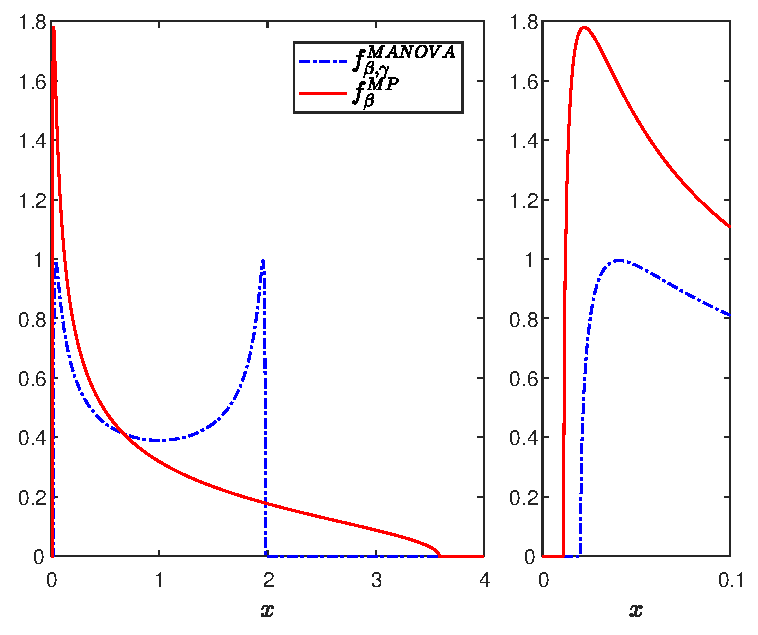
\includegraphics[width=5in]{SpectrumExample_gamma0_5_bata1_25_pnas.eps}
\caption{Limiting 
	MANOVA ($\beta=0.8,\gamma=0.5$) 
% previously beta=1.25
and Mar\u cenko-Pastur ($\beta=0.8$) density
functions. Left: density on the interval $x\in [0,4]$. Right: Zoom in on the
interval $x\in[0,0.1]$. 
%Note that the upper and lower edges of the support of the two densities.....
%\TODO{change plot colors, increase font size everywhere}
}
\label{fig:MANOVA_MP}
\end{figure}

\item {\em Unitary Haar frame:}
Let $X_{haar}^{(n)}$ consist of
the first $\m$ columns of a
Haar-distributed $n$-by-$n$ unitary matrix normalized by $\sqrt{n/\m}$ (the Haar distribution being the
uniform distribution over the group of $n$-by-$n$ unitary matrices).
Edelman and Sutton \cite{Edelman} proved that 
the empirical spectral distribution of $\lambda(\Gk$) also converges, almost
surely in distribution, to the
MANOVA limiting spectral distribution 
(See also \cite{wachter} and the closing remarks of \cite{Farrell}.)
%
\end{enumerate}
%\TODO{new enumeration for e/f/g}
The maximal and minimal eigenvalues of a matrix
from the MANOVA$(n,\m,k,\Fc)$ ensemble ($\Fc\in\left\{ \R,\C \right\}$) 
%$\lambda_{max}(\Gk)$ (resp. $\lambda_{min}(\Gk)$) 
are known to converge almost surely 
to $r_+$ and $r_-$, respectively \cite{Johnstone2008}.
While we are not aware of any parallel results for the random Fourier and Haar
frames,  
the empirical evidence in this paper show that it must be the case.

These random matrix phenomena have practical significance for evaluations of
functions of the form $\specstat(\lambda(\Gk))$ such as those mentioned above.
%\ref{sec:motivation}.
The functions $\specstat_{AC}$ and $\specstat_{Shannon}$, for example, are what \cite{BaiBook}
call {\em linear spectral statistics}, namely functions of $\lambda(\Gk)$ that
may be written as an integral of a scalar function against the empirical measure of $\lambda(\Gk)$.
Convergence of the empirical
distribution of $\lambda(\Gk^{(n)})$ to the limiting 
MANOVA distribution with density $f^{MANOVA}_{\beta,\gamma}$ 
implies %\TODO{$\lambda(\Xkn^{(n)}) \Rightarrow \lambda(\Gkn^{(n)})$}
\begin{eqnarray} \label{ac_limit:eq}
%\lim_{n\to\infty} \specstat_{AC}(\lambda(\Gkn^{(n)})) &=& \beta \int \frac{1}{x}
%\,f_{\beta,\gamma}^{MANOVA}(x)dx \\
\lim_{n\to\infty} \specstat_{AC}(\lambda(\Gkn^{(n)})) &=& \int \frac{1}{x}
\,f_{\beta,\gamma}^{MANOVA}(x)dx \\
\lim_{n\to\infty} \specstat_{Shannon}(\lambda(\Gkn^{(n)})) &=&  \int \log(1+\alpha x)
\,f_{\beta,\gamma}^{MANOVA}(x)dx \nonumber 
\end{eqnarray}
%\TODO{$F_{AC}$ needs a normalization by $\beta$ or $1/\beta$}
for both the random Fourier and Haar frames; 
the integrals on the right hand side may be evaluated explicitly.
Similarly, convergence of 
$\lambda_{max}(\Gk)$ and $\lambda_{min}(\Gk)$ to $r_+$ and $r_-$ implies, for
example, that 
\begin{eqnarray} \label{rip_limit:eq}
\lim_{n\to\infty} \specstat_{RIP}(\lambda(\Gk^{(n)})) = \max(r_+-1,1-r_-)\,.
\end{eqnarray}

To demonstrate why such calculations are significant,
we note that Equations \eqref{ac_limit:eq} and \eqref{rip_limit:eq} 
immediately allow us to compare the Gaussian i.i.d frame
with the random Fourier and Haar frames, 
in terms
of their limiting value of functions of interest.
Figure \ref{fig:limiting_F} compares the limiting value of $\specstat_{RIP}$,
$\specstat_{AC}$ and $\specstat_{Shannon}$ over varying values of $\beta=\lim_{n\to \infty}
k/\m$. The plots 
clearly demonstrate that frames whose typical
$k$-submatrix exhibits a MANOVA spectrum, are superior to frames whose typical
$k$-submatrix exhibits a Mar\u cenko-Pastur spectrum, 
across the performance measures.


\begin{figure*}[h!]
\centering
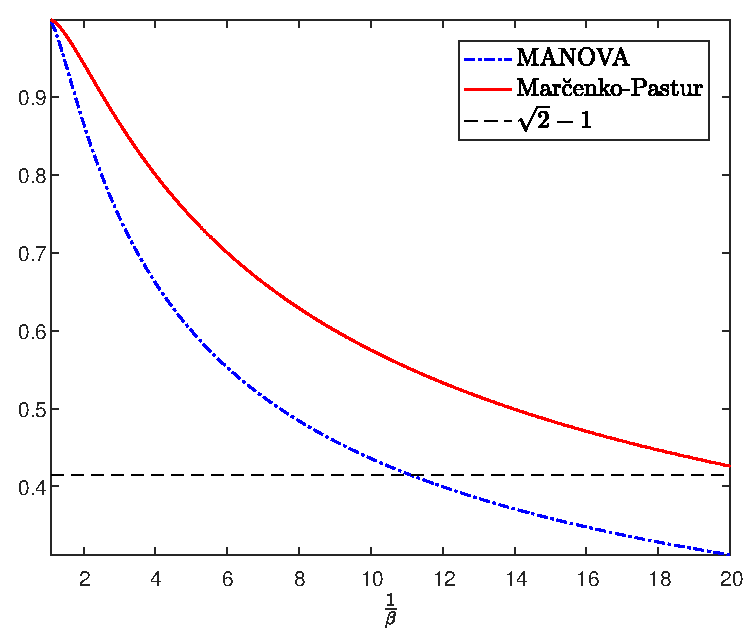
\includegraphics[width=3in]{RIPLimit_gamma0_5_2_pnas.eps}\\
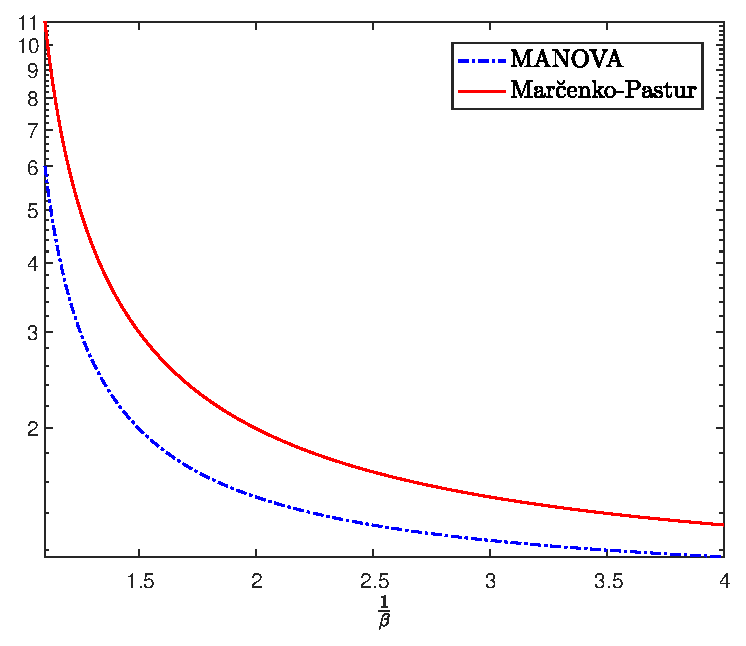
\includegraphics[width=3in]{ACLimit_gamma0_5_2_pnas.eps}\\
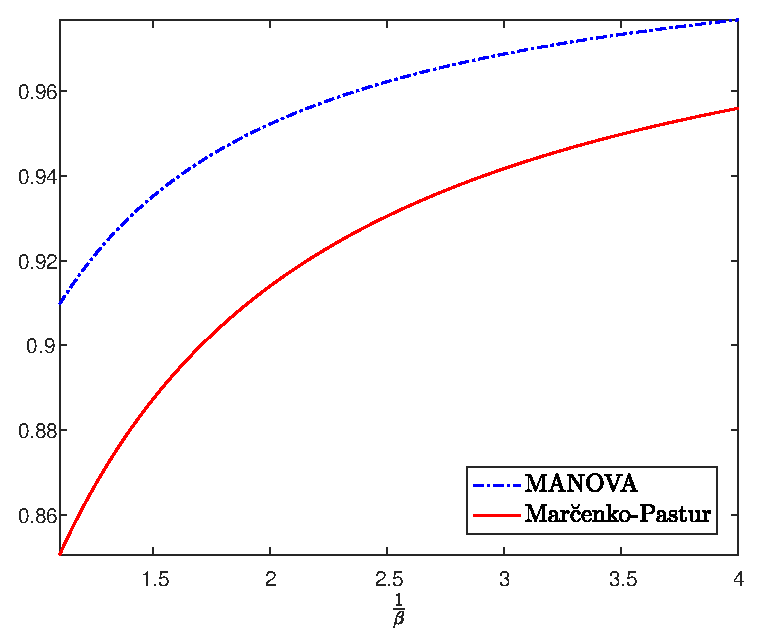
\includegraphics[width=3in]{ShannonLimit_gamma0_5_2_pnas.eps}
\caption{Comparison of limiting values of $\E_K \specstat(\lambda(G_K))$ for the three
functions $\specstat$ discussed in Motivation Section between the Mar\u cenko-Pastur limiting distribution and the MANOVA
distribution. Left: $\specstat_{RIP}$ (lower is better). 
Middle: $\specstat_{AC}$ (lower is
better). Right: $\specstat_{Shannon}$ (higher is better).
%
}
\label{fig:limiting_F}
\end{figure*}


% TODO: from here

%You should let X_K denote the matrix formed by K columns
%and let G_K denote the Gram matrix.
%
%You should let F_{G_{k,n}} denote the empirical spectral distribution of G
%and the \Psi(G_{k,n}) denote the linear spectral statistic. By the way
%the benefit of invoking a connection to linear spectral statistic is minimal
%since you are not invoking the Bai-Silverstein theorem.  It's in fact jus
%a linear functional of the empirical eigenvalue CDF.
%
%You should let
%
%\Psi(F) = \int \psi(x) dF(x)
%
%so that\Psi is the linear functional and \psi(x) is the kernel
%of the functional.
%
%You shouldn't call \Psi a function. It
%is a functional.

%%%%%%%%%%%%%%%%%%%%%%%%%%%%%%%%%%%%%%%%%%%%%%%%%%%%%%%%%%%%%%%%%

\section*{Deterministic Frames: Universality Hypothesis}
\label{sec:deterministic_frames}

Deterministic frames, namely
frames whose design involves no randomness, have so far eluded this kind of
asymptotically exact analysis. 
%shown in Section \ref{sec:random_frames}. 
While
there are results regarding RIP \cite{Bandiera,Fickus} and statistical RIP
\cite{Caulderbank-STRIP,Gurevich2009,Mazumdar}, for example, of deterministic
frame designs, they are mostly focused on highly redundant frames ($\gamma \rightarrow 0$)
and the wide submatrix ($\beta \rightarrow 0$) case, where the spectrum tends
to the Mar\u cenko-Pastur distribution. Furthermore, nothing analogous, say, to the precise comparisons of Figure
\ref{fig:limiting_F} exists in the literature to the best of our knowledge. 
Specifically, no results analogous to \eqref{ac_limit:eq} and \eqref{rip_limit:eq}
are known for deterministic frames, 
let alone the associated convergence rates, if any.

In order to subject deterministic frames to an asymptotic analysis, we shift our
focus from a single frame $X$ to a family of deterministic frames $\{X^{(n)}\}$
created by a common construction. The frame matrix $X^{(n)}$ is $n$-by-$m$.
Each frame family determines allowable sub-sequences $(n,m)$; to
simplify notation, we leave the subsequence implicit and index the frame
sequence simply by $n$. The frame family
also determines the aspect ratio limit $\gamma=\lim_{n\to\infty} \m/n$.
In what follows we also fix a sequence $k$ with $\beta=\lim_{n\to\infty}
k/\m $,
and let $K\subset [n]$ denote a uniformly distributed random subset.

\paragraph{Frames under study.} 

The different frames that we studied are listed in Table \ref{FramesTable},
in a manner inspired by \cite{Monajemi}.
In addition to our deterministic frames of interest 
(the set ${\cal X}$),
the table contains also two examples of random frames
(real and complex variant for each), 
for validation and convergence analysis purposes.
%
%TODO{In table: complete missing entries, check R or C, complete rest, add RandDCT? add DG?}
\begin{table*}[t]
\centering
\caption{Frames under study}
\label{FramesTable}
{\scriptsize
\begin{tabular}{lllllll}
\toprule
Label & Name & $\R$ or $\C$ & Natural $\gamma$ & Tight frame &
Equiangular & References \\
\midrule
& & & & &  & \\
{\bf Deterministic frames} & & & & &  & \\
DSS & Difference-set spectrum & $\C$  & & Yes & Yes & \cite{WBdss}\\
GF & Grassmannian frame & $\C$ & $1/2$& Yes & Yes &  \cite[Cor. 2.6b]{Grassmannian}
\\
RealPF & Real Paley's construction & $\R$ & $1/2$ & Yes & Yes & \cite[Cor. 2.6a]{Grassmannian}
\\
ComplexPF & Complex Paley's construction & $\C$ & $1/2$ & Yes & Yes & 
\cite{PaleyConstruction}
\\
Alltop & Quadratic Phase Chirp & $\C$ & $1/L$ & Yes & No &  
\cite[eq. S4]{Monajemi} with $L=2$
\\
SS & Spikes and Sines & $\C$ & $1/2$ & Yes & No & \cite{Elad2010} \\
SH & Spikes and Hadamard & $\R$  & $1/2$ & Yes & No & \cite{Elad2010}
~ \\\hline  ~\\
{\bf Random frames} & & & & &  & \\
HAAR %\TODO{replace  U-HAAR?}
& Unitary Haar frame & $\C$ & & Yes & No & \cite{Farrell,Edelman} \\
RealHAAR %\TODO{replace  O-HAAR?}
& Orthogonal Haar frame & $\R$ & & Yes & No & \cite{Edelman} \\
RandDFT  %\TODO{replace  RandDFT?}
& Random Fourier transform & $\C$ & & Yes & No & \cite{Farrell} \\
RandDCT  %\TODO{replace  RandDCT?}
& Random Cosine transform & $\R$ & & Yes & No &  \\

\bottomrule
\end{tabular}
}
\label{frames:tab}
\end{table*}

%\TODO{Not any deterministic frame is "good",
%i.e., obeys our universal hypotheses below.}
%\TODO{to give the example of a lowpass frame}

\paragraph{Functionals under study.}

We studied the functionals $\specstat_{StRIP}$ from \eqref{strip_func:eq}, 
$\specstat_{AC}$ from \eqref{ac_func:eq}, $\specstat_{Shannon}$ from
\eqref{shannon_func:eq}. In addition, we studied the maximal and minimal
eigenvalues of $\Gk$, and its condition number:
\begin{eqnarray*}
\specstat_{max}(\lambda(\Gk)) &=&  \lambda_{max}(\Gk) \\
\specstat_{min}(\lambda(\Gk)) &=&  \lambda_{min}(\Gk) \\
\specstat_{cond}(\lambda(\Gk)) &=&  \lambda_{max}(\Gk) / \lambda_{min}(\Gk)\,. 
\end{eqnarray*}



\paragraph{Measuring the rate of convergence.}
%
In order to quantify the rate of convergence of the entire spectrum 
of the $k$-by-$\m$ matrix 
$\Xk$, which is a $k$-submatrix of an $n$-by-$\m$ frame matrix $X$, to a limiting
distribution, we let $F[\Xk]$ denote the
empirical cumulative distribution function (CDF) of $\lambda(\Gk)$, and 
let $F^{MANOVA}_{\beta,\gamma}(x) = \intop_{r_-}^x
f^{MANOVA}_{\beta,\gamma}(x)dx$ denote the CDF of the MANOVA$(\beta,\gamma)$
limiting distribution. 
%\TODO{again, we need MANOVA$(\beta,\gamma,\R)$ -  
%When $\Xk$ is real we compare to MANOVA$(\beta,\gamma,\R)$ etc}.
The quantity
%\TODO{change $k/m$ to $\beta_n$ and also $\gamma$}
\[
\Delta_{KS}(\Xk) = \norm{F[\Xk] - F^{MANOVA}_{\beta_n,\gamma_n}}_{KS}\,,
\]
where $\norm{\cdot}_{KS}$ is the Kolmogorov-Smirnov (KS) distance between CDFs, 
measures the distance to the hypothesised limit. Here, 
$\beta_n=k/m$ and $\gamma_n=m/n$ are the actual aspect ratios for the matrix $\Xk$ at hand.
As a baseline we use $\Delta_{KS}( Y_{n,\m,k,\Fc})$, where 
$Y_{n,\m,k,\Fc}$ is a matrix from the MANOVA$(n,\m,k,\Fc)$ ensemble,
with $\Fc=\R$ if $X_K$ is real and $\Fc=\C$ if complex.
Figure \ref{fig:CDFs} illustrates the KS-distance 
between an empirical CDF and the limiting MANOVA CDF.

\begin{figure}[h]
\centering
\includegraphics[width=5in]
{KSdistance_RScdf_MANOVAcdf_n100_2_pnas.eps}
\caption{KS-distance of random DFT subframe, $\beta = 0.8$, $\gamma = 0.5$, $n=100$.}
\label{fig:CDFs}
\end{figure}

Similarly, in order to quantify the rate of convergence of a functional
$\specstat$, the quantity
\[
\Delta_\specstat(\Xk;n,\m,k) = \big| \Psi(\lambda(\Gk)) -
\Psi(f^{MANOVA}_{\beta_n,\gamma_n}) \big|
\]
is the distance between the measured value of $\Psi$ on a given $k$-submatrix
$\Xk$ and its hypothesised limiting value. 
For a baseline we can use $\Delta_\specstat(Y_{n,\m,k,\Fc})$,
with $\Fc=\R$ if $X_K$ is real and $\Fc=\C$ if complex.
For linear spectral functionals 
like $\Psi_{AC}$ and $\Psi_{Shannon}$, which may be written as
$\Psi(\lambda(\Gk))=\int \psi dF[X_K]$ for some kernel $\psi$, we have
$  \Psi(f^{MANOVA}_{\beta,\gamma}) = \int \psi dF^{MANOVA}_{\beta,\gamma}$. 
For $\Psi_{RIP}$ that depends on $\lambda_{max}(\Gk)$ 
and $\lambda_{min}(\Gk)$ we have $\Psi_{RIP}(f^{MANOVA}_{\beta,\gamma}) =
\max\left\{ r_+-1,1-r_- \right\}$.

\paragraph{Universality Hypothesis.} 

The contributions of this paper are based on the following assertions on the typical $k$-submatrix ensemble $\Xk$ corresponding to a frame
family $X^{(n)}$. This family may be random or deterministic, real or complex. 
%\TODO{need to compare real to real MANOVA and cplx to cplx MANOVA!}

\begin{enumerate}
\item[{\bf H1}] {\em Existence of a limiting spectral distribution.} 
%The typical $k$-submatrix $\Xk$ is a random matrix ensemble with a
%compactly-supported limiting spectral distribution. Formally, 
%The typical $k_n$-submatrix $\Xkn^{(n)}$ is a random
%matrix ensemble with a compactly-supported limiting spectral distribution, 
%as $k/m\to\beta$ and $\m/n\to\gamma$.
The empirical spectral distribution of $\Xk^{(n)}$, namely the 
distribution of $\lambda(\Gk^{(n)})$, converges, as $n\to \infty$, 
to a compactly-supported limiting distribution; furthermore, 
$\lambda_{max}(\Gk^{(n)})$ and $\lambda_{min}(\Gk^{(n)})$ converge to the
edges of that compact support.

\item[{\bf H2}] {\em Universality of the limiting spectral distribution.} 
The limiting 
spectral distribution of $\Xk^{(n)}$ is the 
MANOVA$(\beta,\gamma)$ distribution  \cite{wachter} whose density is 
\eqref{ManovaDensity}. Also 
$\lambda_{max}(\Gk^{(n)})\to r_+$ and $\lambda_{min}(\Gk^{(n)})\to r_-$
where $r_\pm$ is given by \eqref{ManovaDensityExtrimalValues}.


%  A large variety of frames share a common,
%  {\em universal} limiting distribution, which is non other than 
%  Wachter's classical 
%  MANOVA$(\beta,\gamma)$
%  limiting distribution \cite{wachter}.

\item[{\bf H3}] {\em Exact power-law rate of convergence for the entire
spectrum.}
%    For each frame there is an exact power-law rate of
%    convergence of the empirical spectral distribution  to its
%  MANOVA$(\beta,\gamma)$ limit, with a known exponent. 
%  The same hold true for the classical MANOVA (Jacobi) random matrix ensemble
%  \cite{?}.
The spectrum of $\Xk^{(n)}$ converges to the limiting
MANOVA$(\beta,\gamma)$ distribution
\begin{eqnarray*} 
   \left(\E_{K_n}\left(\Delta_{KS}(\Xk^{(n)})\right)\right)^2 \searrow 0
\end{eqnarray*}
and in fact its fluctuations are given by the law
\begin{eqnarray} \label{KS_conv:eq}
Var_{K}(\Delta_{KS}(\Xk^{(n)}))=Cn^{-2b} 
\end{eqnarray}
for some constants $C,b$, which may depend on the frame family.
%   While the constant $C$ may depend on the frame family, 
%   the exponent $b$ is universal and depends only on $\beta$ and $\gamma$.

\item[{\bf H4}] {\em Universality of the rate of convergence for the
entire spectrum of ETFs.}
For an equiangular tight frame (ETF) family,  
the exponent
$b$ in \eqref{KS_conv:eq} is universal and does not depend on the frame. 
Furthermore, 
% \begin{eqnarray*} 
%   \E_{K_n}(\Delta_{KS}(Y_{n,\m_n,k_n} ; n,\m_n,k_n)^2)=Cn^{-b} \,,
%\end{eqnarray*}
\eqref{KS_conv:eq} also holds, with the same universal exponent,
replacing $\Gk^{(n)}$ with a same-sized matrix
from the MANOVA$(n,\m,k,\Fc)$ distribution 
defined in \eqref{ManovaRandomMatrix}, with $\Fc=\R$ if $X^{(n)}$ is a real
frame family, and $\Fc=\C$ if complex. %\TODO{verify} 
%\TODO{R vs R, C vs C}
In other words, the universal exponent $b$ for ETFs 
is a property of the MANOVA
(Jacobi) random matrix ensemble.


%In this sense, 
%the typical $k$-submatrix of various deterministic ETFs 
%is indistinguishable from a MANOVA (Jacobi)
%random matrix of the same size. 

\item[{\bf H5}] {\em Exact power-law rate of convergence for functionals.}
For a ``nice'' functional $\specstat$, the value of
$\specstat(\lambda(\Gk^{(n)}))$  converges
to $\specstat(f^{MANOVA}_{\beta,\gamma})$ according to the law
\begin{eqnarray} \label{func_conv:eq}
\E_{K}(\Delta_\specstat(\Xk^{(n)})^2)=Cn^{-b}\log^{-a}(n)
\end{eqnarray}
%\TODO{log a or -a?}
for some constants $C,b,a$.
% that may depend on the frame.
% SEE NEXT HYPOTHESIS FOR THE CONSTANTS UNIVERSALITY.


%  with a specific power-law rate of convergence. The exponent of
%  $\Psi$ on each frame is known.
\item[{\bf H6}]  {\em Universality of the rate of convergence for functionals.}
While the constant $C$ in \eqref{func_conv:eq} may depend on the frame,
the exponents 
$a,b$ are universal. \eqref{func_conv:eq} 
also holds, with the same universal exponents, 
replacing $\Gk^{(n)}$ with a same-sized matrix 
from the MANOVA$(n,\m,k,\Fc)$ ensemble 
defined in \eqref{ManovaRandomMatrix}, with  
$\Fc=\R$ if $X^{(n)}$ is a real
frame family, and $\Fc=\C$ if complex. 
In other words, the universal exponents $a,b$ 
are a property of the MANOVA
(Jacobi) random matrix ensemble.


%  The exponents of
%  the power law for $\specstat$ on each frame are 
%  identical to the exponent of $\specstat$ on the MANOVA (Jacobi)
%  random matrix.

\end{enumerate}



%\paragraph{Primary conjectures.}
%
%\begin{enumerate}
%  \item The spectral distribution converges to the limiting MANOVA
%  \item The edge spectrum converges to edges of MANOVA
%  \item The flactuations about the limit are $C\cdot n^\alpha$
%  \item For functional, the limit is the functional acting on MANOVA
%  \item The flactuations are \ldots
%\end{enumerate}<++>

%In the reminder of this paper we provide
%compelling empirical evidence, analyzed by statistical
%tests,
%which unanimously
%support the following  conjectures. 
%\begin{center} 
%	   \begin{enumerate}
%      \item[(P1)] {\em The typical submatrix ensemble has a limiting spectral
%        distribution.} Let $\{X^{(n)}\}$ a frame family 
%        under study. 
%        Let $\left\{ k_n \right\}$ be a sequence 
%        with 
%        $k_n/\m_n \to \beta$ and let $K_n$ be a uniformly random 
%        subset of $[n]$. 
%        The ensemble $\Xkn^{(n)}$ behaves like a classical random matrix
%        ensemble in the following sense:
%        %Almost surely, 
%        The empirical distribution of the 
%        spectrum $\lambda(\Xkn)$
%        converges, 
%        %in distribution, 
%        as $n\to\infty$, to a compactly supported 
%        limiting distribution. Furthermore, the maximal and minimal eigenvalues
%        $\lambda_{max}(\Gkn)$ and 
%        $\lambda_{min}(\Gkn)$
%        converge 
%        %in probability 
%        to the edges of the compact support.
%
%      \item[(P2)] {\em Universality of the limiting spectral distribution.}
%        Let $\{X^{(n)}\}$ be a frame family under study. Then the limiting
%        spectral distribution of $\Xkn^{(n)}$ is the 
%        MANOVA$(\beta,\gamma)$ distribution whose density is 
%        \eqref{ManovaDensity}. Also 
%        $\lambda_{max}(\Xkn)\to r_+$ and $\lambda_{min}(\Xkn)\to r_-$
%        where $r_\pm$ is given by \eqref{ManovaDensityExtrimalValues}.
%      %
%      \item[(P3)] {\em Universality of the convergence rate of the spectrum CDF.}
%        Let $\{X^{(n)}\}$ a frame family 
%        under study and 
%        let $\Delta(KS,n)$ be the Kolmogorov-Smirnov distance between the
%        empirical spectral distribution of $\Xkn^{(n)}$ and the cumulative
%        distribution
%        function corresponding to the MANOVA$(\beta,\gamma)$ density
%        \eqref{ManovaDensity}. Then
%        $\lim_{n\to\infty} \E_{K_n}(\Delta(KS,n)^2)=0$ and in fact
%         $\E_{K_n}(\Delta(KS,n)^2)=Cn^{-b}$ for some constants $C,b$ 
%        that depend on the frame. The constant $b$ is equal for the classical
%        MANOVA random matrix ensemble \eqref{ManovaRandomMatrix} 
%        and for the frame family. 
%
%      \item[(P4)] {\em Universality of the convergence rate of spectral
%        functionals.}
%        Let $\{X^{(n)}\}$ a frame family 
%        under study and 
%        let $\specstat(\lambda(\Gk))$ be one a functional of the spectrum of
%        $\Gk$
%        mentioned above: $\specstat_{RIP}$, $\specstat_{AC}$ and 
%        $\specstat_{Shannon}$. \TODO{add others}
%        Also let $\specstat_\infty$ be its limiting value on the corresponding 
%        limiting MANOVA$(\beta,\gamma)$ density from
%        \eqref{ManovaDensity}. Define $\Delta(\specstat,n)=| \specstat(\lambda(\Gkn))
%        -\specstat_\infty|$.
%         Then
%        $\lim_{n\to\infty} \E_{K_n}(\Delta(\specstat,n)^2)=0$ and in fact
%         $\E_{K_n}(\Delta(\specstat,n)^2)=Cn^{-b}\log^a(n)$ 
%         for some constants $C,b,a$ 
%        that depend on the frame. The constants $a,b$ are equal for the classical
%        MANOVA random matrix ensemble \eqref{ManovaRandomMatrix} 
%         and for the frame family. 
%
%         \TODO{this is too formal. can we write something like ``identity of the
%         limit and rates of convergence''?}
%
%
%%        $F_K$ is indistinguishable from the spectrum of a MANOVA random
%%matrix of the same size.
%\end{enumerate}
%
%\end{center}
%
%\TODO{Dave suggests that we make this less mathematical.}
\paragraph{Nonstandard aspect ratio $\beta>1$.}
While the classical MANOVA ensemble and limiting density are not defined for
$\beta>1$, in our case it is certainly possible to sample $k>m$ vectors from the
$n$ possible frame vectors, resulting in a situation with $\beta>1$.
In this situation, the hypotheses above require slight modifications.
Specifically, the limiting 
spectral distribution of $\Xk^{(n)}$, for $\beta>1$, is
%\begin{equation}
%\label{ManovaDensityBeta}
%	\begin{aligned}
%&(1-\frac{1}{\beta})\delta(x)+\frac{1}{\beta^2}f_{\frac{1}{\beta},\beta\gamma}^{MANOVA}(\frac{1}{\beta}x)\\
%& =(1-\frac{1}{\beta})\delta(x)+f_{\beta,\gamma}^{MANOVA}(x)\,,
%	\end{aligned}
%\end{equation}
\begin{equation}
\label{ManovaDensityBeta}
	\left(1-\frac{1}{\beta}\right) \delta(x)+f_{\beta,\gamma}^{MANOVA}(x)\,,
\end{equation}
where $f_{\beta,\gamma}^{MANOVA}(x)$ is the function (no longer a density) 
defined in \eqref{ManovaDensity}.
%but not in the sense of density, as MANOVA density and ensemble are defined only for $\beta<1$.
The rate of convergence of the distribution of nonzero eigenvalues to the
limiting density
$\frac{1}{\beta}f_{\frac{1}{\beta},\beta\gamma}^{MANOVA}(\frac{1}{\beta}x)=\beta
f_{\beta,\gamma}^{MANOVA}(x)$ is compared with 
the baseline $\beta\cdot Y_{n,k,\m,\Fc}$, where $Y_{n,k,\m,\Fc}$ is a matrix from the MANOVA$(n,k,\m,\Fc)$ ensemble
(i.e., with reversed order of $k$ and $m$).
%\TODO{maybe define $(1-\frac{1}{\beta})_+\delta(x)+f_{\beta,\gamma}^{MANOVA}(x)$ in the beginning as the limiting density for every $\beta$}
%\TODO{claim also the power law hypothesis without simulating or only the limit which we are sure of?}

%%%%%%%%%%%%%%%%%%%%%%%%%%%%%%%%%%%%%%%%%%%%%%%%%%%%%%%%%%%%%%%%%%%%

% BEGIN SMALL FOR RESULTS

\section*{Methods} \label{sec:methods}

The software we developed has been permanently deposited 
in the Data and Code Supplement \cite{SDR}.
As many of the deterministic frames under study are only defined for $\gamma=0.5$, 
we primarily studied the aspect ratios $(\gamma=0.5,\beta)$ with 
$\beta\in\{0.3,0.5,0.6,0.7,0.8,0.9\}$.
%and $(\gamma=0.5,\beta=0.6)$ %TODO{change to 0.8 and 0.6 everywhere including ode, figures}.
%and $1000\leq n \leq 2000$ for most of the frames. For Grassmannian frame and Spikes and Hadamard frame $n$ as large as $4096$ was tested.
In addition, we inspected all frames under study that are defined for the aspect ratios $(\gamma=0.25,\beta=0.6)$ and $(\gamma=0.25,\beta=0.8)$ (all random frames, as well as DSS and Alltop).
%andom frames under 
We also studied nonstandard aspect ratios $\beta>1$ as described in the
Supporting
Information \cite{SI}. 
For deterministic frames, $n$ took allowed values in the range 
$(240,2000)$, $(2^5,2^{12})$ for Grassmannian and Spikes and Hadamard frames and $(600,4000)$ for DSS frame with $\gamma=0.25$.
For random frames and MANOVA ensemble we used
dense grid of values in the range $(240,2000)$. 
Hypothesis testing as discussed below, 
was based on a subset of these values where $n\ge 1000$.
For each of the frame families under study, and for each value of $\beta$ and
$\gamma$ under study, we selected a sequence $(n,\m,k)$.
%with $k/\m_n=\beta$ and $\m_n/n=\gamma$. 
The values $n$ and $m$ were selected so that $m/n$ will be as close as
possible to $\gamma$, however due to different aspect ratio constrains by the
different frames occasionally we had $m/n$ close but not equal to $\gamma$.
We then determined $k$ such that $k/\m$ will be as close as
possible to $\beta$.
For each $n$, we generated a single 
$n$-by-$\m$ frame matrix
$X^{(n)}$.
% (Note that for the deterministic 
%frames we studied, there is no randomness whatsoever in the frame matrix 
%$X^{(n)}$. For random frames, we generated a single random frame from each value
%of $n$.)
We then produced $T$ independent samples from the uniform
distribution on $k_n$-subsets,
$K[1],\ldots,K[T]\subset[n]$, and generated 
their corresponding $k$-submatrices 
$X_{K[i]}^{(n)}$ ($1\leq i\leq T$). Importantly, all these are submatrices of
the same frame matrix $X^{(n)}$.
We calculated $\overline{\Delta}^{Var}_{KS}(\Xk^{(n)})=\overline{\Delta^2}_{KS}(\Xk^{(n)})-\overline{\Delta}^2_{KS}(\Xk^{(n)})$, the empirical variance of 
$ \Delta_{KS}(X_{K[i]}^{(n)})$, and $\overline{\Delta^2}_{KS}(\Xk^{(n)})$, the average value of $ \Delta^2_{KS}(X_{K[i]}^{(n)})$ on $1\leq i\leq T$, as a 
%\[
%  \frac{1}{\kappa}\sum_{i=1}^\kappa \Delta_{KS}(X_{K_n[i]}^{(n)};n,\m_n,k_n)
%\]
monte-carlo approximation  to the left-hand side of \eqref{KS_conv:eq}, variance and MSE respectively. For each
of the functionals under study, we also calculated 
$ \overline{\Delta^2}_\specstat(X_{K[i]}^{(n)})$,
the average value of 
$ \Delta^2_\specstat(X_{K[i]}^{(n)})$ on 
$1\leq i\leq T$, as a monte-carlo approximation to the left-hand size of 
\eqref{func_conv:eq}.

Separately, 
for each triplet ($n$,$m$,$k$) and $\Fc\in\left\{ \R,\C \right\}$
we have performed $T$ independent draws from
the MANOVA$(n,\m,k,\Fc)$ ensembles 
(\ref{ManovaRandomMatrix}) and calculated 
analogous quantities 
$\overline{\Delta}^{Var}_{KS}(Y_{n,\m,k,\Fc})$,
$\overline{\Delta^2}_{KS}(Y_{n,\m,k,\Fc})$ 
and
$\overline{\Delta^2}_{\specstat}(Y_{n,\m,k,\Fc})$.





%Here, {\em Haar Frame} is a random selection of columns from a uniformly distributed random orthogonal
%matrix, {\em Random spectrum} is a uniformly random selection of frequencies
%from a DFT matrix, Difference set spectrum is described in ,
%Grassmannian frame is described in, Paley's
%construction is described in  and 
%, Quadratic Phase Chirp is based on Alltop sequence as described in, Spikes and Sines is the concatenation of and identity matrix and a
%DFT matrix and Spikes and Hadamard is the concatenation of and identity matrix and a
%Hadamard matrix.

%The bottom part of Table \ref{FramesTable} lists random frames. 
%As sanity checks, we generated the random frame matrices
%$F^{(n)}_{fourier}$ and $F^{(n)}_{haar}$. While, as mentioned above, the
%empirical spectral distribution of the typical $k$-submatrix 
%has been proved to converge to
%the limiting MANOVA spectral distribution, nothing is known so far to the best
%of our knowledge regarding the distribution of the typical $k$-submatrix in
%finite $n$. Alongside evidence supporting our Primary Conjecture, we bring
%similar evidence that the finite-$n$ distribution of the typical $k$-submatrix
%of $F^{(n)}_{fourier}$ and $F^{(n)}_{haar}$ is also indistinguishable from a
%MANOVA matrix of the same size.


%For a given choice of $(\beta,\gamma)$, 
%for each frame family under study, and for frame size $n$ allowable by the frame
%family,
%we generated a single frame matrix $F^{(n)}$ of size $n$-by-$m_n$.
%Note that for the deterministic 
%frames we studied, there is no randomness whatsoever in the frame $F^{(n)}$. 
%The values $n$ and $m_n$ were selected so that $m_n/n$ will be as close as
%possible to $\gamma$, however due to different aspect ratio constrains by the
%different frames occasionally we had $m_n/n$ close but not equal to $\gamma$.
%We determined $k_n$ such that $\m_n/k_n=\beta$.
%We then produced $T$ 
%independent samples of $k_n$-subsets $K(1),\ldots,K(T)\subset
%[n]$.
%For each sample, we generated the $k_n$-submatrix $F^{(n)}_{K_n}$ and calculated
%its spectrum $\lambda=\lambda(F^{(n)}_{K_n})$.
%We then calculated the KS distance between the empirical CDF of $\lambda$ and
%the CDF of the limiting MANOVA($m_n/k_n,m_n/n)$ distribution. This yielded $T$
%independent samples of $\Delta(KS,n)$. The mean of these samples was calculated
%and we denote it $\bar{\Delta}(KS,n)$.
%Importantly, these draws came from
%submatrices of the same frame matrix  $F^{(n)}$.

%Testing {\bf P1} and {\bf P2} involves looking at the functions
%\begin{eqnarray*}
%  f_{max}(\lambda(F_K))&=& \lambda_{max}(F_K)\\
%  f_{min}(\lambda(F_K))&=& \lambda_{min}(F_K)\,.
%\end{eqnarray*}
%For each of the functions $f_{RIP}$, $f_{AC}$, $f_{Shannon}$, 
%$f_{max}$, $f_{min}$ we calculated the error $\Delta(f,n)$ and obtained $T$
%independent samples of this quantity. The mean of these samples was calculated
%for each $f$, and we denote it $\bar{\Delta}(f,n)$.
%

%multiple
%submatrices with a uniformly random subset of rows. We subjected the collection
%of submatrices to tests developed in order to compare the collection with a
%collection of i.i.d samples from the corresponding MANOVA ensemble. 
%For each value of $n$ we use $f_{\beta_n,\gamma_n}^{MANOVA}$ as the limiting distribution.
%The reason for slightly different parameters (asymptotically the same) is the different possibles sets of $n$'s for different frames and the constraint on integer matrix dimensions.
%
%It is important to mention that for each value of $n$ (for different frames different sets of $n$'s are possible) the beta is a bit different (asymptotically the same) and the limiting values of the functionals are calculated related to the relevant beta, n/m ratios.
%The limiting minimal/maximal eigenvalues (and the condition number) are based on
%the limits of the support of Manova distribution. \TODO{rephrase}

%\subsection{Test 1: Goodness-of-fit of the entire spectrum}
\paragraph{Test 1: Testing H1--H4.}
%\TODO {$\log$ -> $\ln$}
For each of the frames under study and each value of $(\beta,\gamma)$, we computed the KS-distance for $T=10^4$
submatrices and performed simple linear regression
of 
$-\frac{1}{2}\log\left( \overline{\Delta}^{Var}_{KS}(\Xk^{(n)})\right)$ 
on $\log(n)$ with an intercept. We obtained 
the estimated linear coefficient $\hat{b}$ as an estimate
for the exponent $b$, and its standard error $\sigma(\hat{b})$.
Similarly we regressed 
$-\frac{1}{2}\log\left( 
\overline{\Delta}^{Var}_{KS}(Y_{n,\m,k,\Fc})\right)$
on $\log(n)$ to obtain $\hat{b}_{MANOVA}$ and $\sigma(\hat{b}_{MANOVA})$.  
%Denote by $N$ the number of different values of $n$ for which we have collected
%the data $\bar{\Delta}(KS,n)$ and let $\V{n}$ denote the length-$N$ vectors
%containing these values.
%We neglect the variability in the fitted slope $\hat{b}_{MANOVA}$, which is
%extremely small, and write simply $b_{MANOVA}$ for $\hat{b}_{MANOVA}$.
We performed Student's
t-test to test the null hypotheses $b=b_{MANOVA}$ using
%Specifically, 
%letting $Z$ denote the $N$-by-$2$ regression
%matrix whose columns are $\bf{1}$ and $\log({\V{n}})$, 
the test
statistic 
\[
t = \frac{\hat{b}-b_{MANOVA}}
{\sqrt{\sigma(\hat{b})^2+\sigma(\hat{b}_{MANOVA})^2 }}\,.
\]
%where $(Z'Z)^{-1}_{2,2}$ is the $(2,2)$-th entry of the $2$-by-$2$ matrix
%$(Z'Z)^{-1}$ and where
%\[
%  s = \sqrt{\frac{1}{N-2}\norm{\V{r}}^2}\,.
%\]
%Here, $\V{r}$ is the vector of residuals of the linear fit.
Under the null hypothesis, 
the test statistic is distributed $t_{(N+N_{MANOVA}-4)}$, %\TODO{N-4?} 
where $N$, $N_{MANOVA}$ are the numbers of different values of $n$ for which we have collected
the data for a frame and the MANOVA ensemble respectively.
We report the $R^2$ of
the linear fit; the slope coefficient $\hat{b}$ and its standard error; and the
p-value of the above t-test.
We next regressed $-\log \left(\overline{\Delta^2}_{KS}\right)$ on $\log(n)$. 
Since $\overline{\Delta^2}_{KS} = \left( \overline{\Delta}_{KS}
\right)^2+\overline{\Delta}_{KS}^{Var}$, a linear fit verifies that 
$ \left( \overline{\Delta}_{KS}
\right)^2 \searrow 0$.

%This test involves the KS distance of the 
%entire spectrum of a $k$-submatrix to the conjectured
%limiting MANOVA spectrum. We test the rate of convergence of the variance of 
%this random distance to
%zero as $n$ grows.



%In the first suite of tests we compare the entire spectrum of the submatrix to that
%of a MANOVA matrix. 
%The first hypothesis tested here is simply: ``the limiting spectral distribution
%of $F_K$ is the limiting MANOVA spectral distribution \eqref{ManovaDensity}''.
%To test this hypothesis, one can choose a large enough $n$, draw several
%matrices from $F_K$ (for random $K$) and run a goodness-of-fit test between the
%spectrum of $F_K$ and the CDF corresponding to the density
%\eqref{ManovaDensity}.
%We do more than that. For a given value of $n$, consider the random variable 
%%$W_n=KS\left( \sigma(F^{(n)}_K), \sigma_{MANOVA}\right)$
%$W_n=KS\left( \lambda(F^{(n)}_K), f_{\beta_n,\gamma_n}^{MANOVA}\right)$ where $KS$ is the KS test
%statistic. \comm{$\lambda(F^{(n)}_K)$ or $\sigma^2(F^{(n)}_K)$ ??} \TODO{Marina- just to make sure we compare to the limit and not
%through a two-sample KS. - Yes!} (The simpler suggestion above would correspond to
%checking that $W_n$ lies below some critical value for large $n$. )
%While we are not familiar with a result regarding the rate of convergence of 
%$W_n$ to zero, in similar models $W_n\approx 1/n$, see for example \cite{Gotze}.
%%We expect its standard deviation  to drop faster than $1/\sqrt{n}$.
%\TODO{(Why?)}
%Assuming $std(W_n)\sim\frac{1}{n^b}$, the slope of $-\log(std(KS))$ vs $\log(n)$ should represent the exponent $b$.
%The hypothesis is that this slope is equal between the actual MANOVA draws, and
%the frames. This is a hard test to pass: in order to pass, the empirical
%spectrum of a matrix from the ensemble $F_K$ needs not only to be similar to the
%limiting spectrum, but to converge to this limit exactly as fast as the actual
%MANOVA ensemble does!
%In other words, the hypothesis tested here is: ``The rate of convergence of the\comm{??} 
%%We used the Kolmogorov-Smirnov test for goodness of fit evaluation of 
%We compared the cumulative distribution function (CDF) of the empirical
%eigenvalue distribution of the submatrix to the CDF of the limiting MANOVA
%eigenvalue distribution, namely the CDF corresponding to \eqref{ManovaDensity}.

%For every frame and growing ${n}$, we compute the Kolmogorov-Smirnov (KS) test
%statistic for each realization of random submatrix and calculated its standard
%deviation over many draws of a random submatrix. We expect it to drop faster than $\frac{1}{\sqrt{n}}$. Assuming $std(KS)\sim\frac{1}{n^b}$, the slope of $-\log(std(KS))$ vs $\log(n)$ should represent the exponent $b$.

%As a sanity check, we also drew i.i.d matrices from the actual MANOVA ensemble.
%The exponent $b$ measures the {\em rate of decrease} of the standard deviation
%of the KS distance between the empirical eigenvalue distribution and the
%limiting MANOVA CDF.
%
%Statistical test: we fit a 5-th degree polynomial and test for significance of
%the quadratic and beyond coefs. This is to verify that the model
%$std(W_n)\sim\frac{1}{n^b}$ holds. We report p-value of MANOVA of the linear
%model vs the higher order models. If all curves are found to be linear, we
%extract the exponent $b$ with standard error for each, and report the 
%Z-test
%two-sample
%t-test comparing the coefficient $b$ of each frame with that of the MANOVA
%curve. Specifically, \cite{regression} if $\hat{b}_*$ is the slope coefficient for  
%MANOVA and $\hat{b}_1$ is the slope coefficient for some frame, we use the test
%statistic 
%\[
%  \frac{\hat{b}_1-\hat{b}_*}{\sqrt{SE(\hat{b}_1)^2+SE(\hat{b}_*)^2}}
%\] 
%and report the Z-score and p-value for each frame.
%

%\subsection{Test 2: Test functionals}
\paragraph{Test 2: Testing H5--H6.}

For each of the frames under study, each of the functionals $\specstat$ 
under study, and 
each value of $(\beta,\gamma)$, we computed the empirical value of the
functionals on $T=10^3$ submatrices.
We first performed linear regression
%
%The second suite of tests used test functionals of the empirical CDF. Rather
%than testing the empirical CDF as a whole, it focused on a specific real-valued 
%observable of the empirical CDF.
%
%To test the convergence of the largest and smallest eigenvalues
%(as in {\bf P1} and {\bf P2})  and the convergence rate of spectral functionals 
%(as in {\bf P4})  
%we performed simple linear regression
%of $-\log\left( \bar{\Delta}(f,n) \right)$ 
of 
$-\log\left( \overline{\Delta^2}_{\specstat}(Y_{n,\m,k,\Fc})\right)$
on $\log(n)$ and $\log(\log(n))$ with an intercept, for $\Fc\in\left\{ \R,\C
\right\}$. 
Let $a_0$ denote the fitted coefficient for $\log(n)$ and let $b_0$ denote the
fitted coefficient for $\log(\log(n))$. 
%This
%was performed separately for each of the functions of interest. 
%(The constant $d$ was calculated as a preliminary procedure by 
%regressing  $-\log\left( \bar{\Delta}(f,n) \right)$ for the MANOVA ensemble 
%on $\log(\V{n})$ and $\log(\log(\V{n}))$ to obtain regression coefficients
%$b_0$ and $a_0$. The then let $d=a_0/b_0$.  )
This step was based on triplets $(n,m,k)$ yielding accurate aspect ratios in
the range $240\le n\le 2000$.
%(and not $n\ge 1000$).
We then performed simple linear regression
of 
$-\log\left( \overline{\Delta^2}_{\specstat}(\Xk^{(n)};n,\m,k)\right)$
on 
$\log(n) + (a_0/b_0)\cdot \log(\log(n))$.
The estimated linear regression coefficient $\hat{b}$
is the estimate 
for the exponent $b$ in \eqref{func_conv:eq}, 
and $\sigma(\hat{b})$
is its standard error. We used 
$\hat{b}\cdot(a_0/b_0)$ as an
estimate for the exponent $a$ in
\eqref{func_conv:eq}.
% The estimate $\hat{b}$ of the linear coefficient
%for the exponent $b$ is the slope of the fit and also determines the exponent
%$a$.
We proceeded as above to test the null hypothesis $b=b_0$.
We report the $R^2$ of
the linear fit; the slope coefficient $\hat{b}$ and its standard error; and the
p-value of the test above.

%
%We computed different functionals of the eigenvalues. Examples for interesting functionals: extremal eigenvalues ($\lambda_{min}$,$\lambda_{max}$), condition number ($\frac{\lambda_{max}}{\lambda_{min}}$), $f_{AC}$, $f_{Shannon}$ \TODO{add RIP if ready}. The asymptotic theoretic values can be computed theoretically or empirically from the MANOVA limiting density. For example $f_{AC} \rightarrow \frac{1}{\beta}\E(\lambda^{-1})$. The limiting $\lambda_{min}$,$\lambda_{max}$ (and the condition number) are based on
%the limits of the support of MANOVA distribution.
%
%We verified for each functional that the bias goes to zero with growing $n$, for matrices from MANOVA ensemble as well as for random submatrices of every other studied frame.
%We compared the variance decay (convergence rate) of the structured frames to that of the MANOVA matrices.
%
%Some functionals are linear functionals of the spectrum, and if the empirical
%spectral distribution really does converge to the limiting MANOVA spectral
%distribution, their convergence would follow. Some (for example, $\lambda_{max}$)
%are not linear, and need not a-priori converge to the corresponding quantity
%(bulk edge.) \TODO{explain, connect to previous TODO}

%We expect the variance to behave like $n^\alpha \log^\beta(n)$. \TODO{why?}
%to find the coefficient $\beta/\alpha$ we regress the log variance for MANOVA on 
%the variables $\alpha \cdot \log(n)$ and $\beta\cdot \log(\log(n))$ (and an
%intercept) to estimate $\alpha$ and $\beta$. We then plot for
%each frame $\log(var)$ over $\log(n)+\hat{\beta}/\hat{\alpha} \log(\log(n))$. 
%We repeat the analysis from test 1: test for linearity in each plot, and then
%test for equality of the slopes.
%\TODO{use different constants, $\beta$, $\gamma$ already used}


% TAKING OUT TRACY WIDOM -------
%  \subsection{Test 3: Tracy-Widom laws}
%  \TODO{does this stay in this paper??}
%  For many different random matrix models, in which the empirical spectral
%  distribution converges to a limiting spectral distribution with compact support,
%  the largest empirical eigenvalue $\lambda_{max}$ converges to the supremum of the
%  support of the limiting spectral distribution. In many of these models, the
%  small fluctuations of $\lambda_{max}$ about this limiting value  have a known
%  distribution, in the sense that there are sequences $\mu_n$ and $\sigma_n$ such
%  that $(\lambda_{max}-\mu_n)/\sigma_n$ converges in distribution to a limiting
%  distribution known as the Tracy-Widom distribution $F_1$. For the MANOVA case,
%  this has been proved by Johnstone \cite{Johnstone2008}. We test the hypothesis:
%  ``using the same scaling $\mu_n$ and $\sigma_n$ as the MANOVA ensemble, the
%  distribution of $\lambda_{max}$ is approximately $F_1$.'' 
%  Note that this is a high-precision test: the top singular value of $F_K$,
%  centered and rescaled using the same relations of MANOVA, need to be $F_1$. 
%  We draw a sample of matrices $F_K$ and compute the TW statistic for each one. We
%  then use a goodness of fit test, KS, to test the fit to $F_1$.
%  We report the test statsitic, p-value, and also plot the CDFs and show a q-q
%  plot. 
% \TODO{maybe change $\sigma_n$ to some other notation?, $F_1$ for real case...}
% -----------

\paragraph{Computing.}

To allow the number of monte-carlo samples to be as large as $T=10^4$ 
and $n$ to be as large as $2000$, we used a large Matlab cluster 
running on Amazon Web Services.
We used 32-logical core machines, with 240GB RAM each, 
which were running several hundred hours in total. 
%The work was distributed to 128 workers, meaning 16 workers per a machine.
The code we executed has been
deposited \cite{SDR}; it
may easily be executed for smaller values of $T$ and $n$ on smaller machines.


% END SMALL FOR RESULTS

%%%%%%%%%%%%%%%%%%%%%%%%%%%%%%%%%%%%%%%%%%%%%%%%

\section*{Results} \label{sec:results}

The raw results obtained in our experiments, as well as the analysis results 
of each experiment, have been deposited with their generating code \cite{SDR}.

%The data we obtained in our experiments has been deposited \cite{SDR}.
%code and experimental data has been deposited \cite{SDR}.
For space considerations, the full documentation of our
results is deferred to the
Supporting Information \cite{SI}.
To offer a few examples,
Figure \ref{fig:KS1} and Table \ref{tab:KS1} show the linear fit to $\overline{\Delta}^{Var}_{KS}$ for  $(\gamma=0.5,\beta=0.8)$.
Figure \ref{fig:KS2} % and Table \ref{tab:KS2} 
shows the linear fit to
$\overline{\Delta}^{Var}_{KS}$ for a different value of $\beta$, namely  $(\gamma=0.5,\beta=0.6)$.
%Figure \ref{fig:KS_MSE1} and Table \ref{tab:KS_MSE1} show the linear fit to $\overline{\Delta^2}_{KS}$ for  $(\beta,\gamma)=(0.8,0.5)$. 
%Figure \ref{fig:f_RIP} and Table \ref{tab:f_RIP} show the linear fit to
%$\overline{\Delta}_{\specstat_{StRIP}}$ for  $(\gamma=0.5,\beta=0.8)$. 
Figure \ref{fig:f_AC} %and Table \ref{tab:f_AC} 
shows the linear fit to
$\overline{\Delta}_{\specstat_{AC}}$ for  $(\gamma=0.5,\beta=0.8)$.
Figure \ref{fig:f_Shannon} and Table \ref{tab:f_Shannon} show the linear fit to
$\overline{\Delta}_{\specstat_{Shannon}}$ for  $(\gamma=0.5,\beta=0.8)$. Similar figures and tables for the other values $(\gamma,\beta)$, in particular, $(\beta=0.3,\gamma=0.5)$, $(\beta=0.5,\gamma=0.5)$,  $(\beta=0.7,\gamma=0.5)$,  $(\beta=0.9,\gamma=0.5)$, $(\beta=0.6,\gamma=0.25)$, $(\beta=0.8,\gamma=0.25)$, are deferred to the Supporting Information. 
%Figure \ref{fig:f_Max} and Table \ref{tab:f_Max} show the linear fit to
%$\overline{\Delta}_{\specstat_{\lambda_{max}}}$ for  $(\beta,\gamma)=(0.8,0.5)$. Figure \ref{fig:f_Min} and Table \ref{tab:f_Min} show the linear fit to
%$\overline{\Delta}_{\specstat_{\lambda_{min}}}$ for  $(\beta,\gamma)=(0.8,0.5)$.
%(Being universal, these estimates are not specific to any particular frame.)
Note that in all coefficient tables, both those shown here and those deferred to the
Supporting Information, upper box shows complex frames (with t-test comparison
to the complex MANOVA ensemble of the same size,
denoted ``MANOVA'') and bottom box shows 
real frames (with t-test comparison to the real MANOVA ensemble of the same
size, denoted ``RealMANOVA'').
In each box, top rows are deterministic frames and bottom rows are random
frames.  Further note that in plots for Test 2 the horizontal axis is slightly
different for real and complex frames, as the preliminary step described above
was performed separately for real and complex frames. In the interest of space,
we plot all frames over the horizontal axis calculated for complex frames.

\paragraph{Validation on random frames.}
While our primary interest was in deterministic frames, we included in the
frames under study random frames. For the complex Haar frame and random Fourier
frame, convergence of the empirical CDF of the spectrum to the limiting
MANOVA$(\beta,\gamma)$ distribution has been proved in
\cite{Farrell,Edelman}. To our surprise, not only was our framework validated on
the four random frames under study, in the sense of asymptotic empirical spectral
distribution, but all universality hypotheses {\bf H1--H6} were accepted (not
rejected at the 0.001 significance level, with very few exceptions).

\paragraph{Test results on deterministic frames.}
A tabular summary of our results, per hypothesis and per frame under study, is included for convenience in the Supporting Information. 
Universality Hypotheses {\bf H1--H3} were accepted on all deterministic frames.
for {\bf H1--H2}, 
convergence of the empirical spectral distribution to the MANOVA$(\beta,\gamma)$
limit has been observed in all cases. For {\bf H3}, the linear fit in all cases
was excellent with $R^2>0.99$ without exception, confirming the power law 
in \eqref{KS_conv:eq} and the polynomial 
decrease of $\overline{\Delta^2}_{KS}$
with $n$.
Universality Hypothesis {\bf H4} was accepted (not rejected) for deterministic
equiangular tight
frames (ETFs) %\TODO{what about real PF?} 
at the 0.001 significance level, with few exceptions (see Table \ref{tab:KS1} below, as well as full results and summary table in the Supporting Information); it was rejected for
deterministic non-ETFs. For $\gamma=0.25$, Hypothesis {\bf H4} has also been accepted for the Alltop frame, see Supporting Information.  
Universality Hypothesis {\bf H5} was accepted for all deterministic frames, with
excellent linear fits ($R^2>0.97$ without exception), confirming the power law
in  \eqref{func_conv:eq}.
Universality Hypothesis {\bf H6} was accepted (not rejected) at the 0.001
significance level (and even 0.05 with few exceptions) for all deterministic frames.
%
For the reader's convenience, 
Table \ref{ExpSummary} summarizes the universal
exponents for convergence of the entire
spectrum ({\bf H4}) and the universal exponents for convergence of 
the functionals under study ({\bf H6}), for $(\beta,\gamma)=(0.8,0.5)$.
The framework developed in this paper readily allows tabulation of these new
universal exponents for any value of $(\beta,\gamma)$.
%
We have observed that the universal exponents are slightly sensitive to the random seed. However, exact evaluation of this variability requires very significant computational resources and is beyond our present scope. Similarly, some sensitivity of the p-values to random seed has been observed.
% and $(\beta,\gamma)=??$.


%We note the following:
%\begin{itemize}
%\item In all figures and tables below "MANOVA" relates to ensemble, tests are preformed on matrix $Y_{n,m,k}$ as described in Section \ref{sec:methods}. 
%\end{itemize}
%Convergence of the entire spectrum:
%\begin{itemize}
%\item The high values of $R^2$ in Table \ref{tab:KS_MSE1} approve that the spectrum converges to the limiting
%MANOVA$(\beta,\gamma)$ distribution with the exact power-law rate for all frames under study.
%\item The null hypothesis $b=b_{MANOVA}$ is not rejected for
%the deterministic ETF frames DSS, GF, RealPF, CoplexPF as well as for random frames HAAR, RealHAAR, RandDCT and RandDFT. 
%\item We tested also on $\beta=0.6$ in order to verify that the hypothesis hold on more then one value of $\beta$. Similar behavior is observed. All results are available in the Supporting Information.  \TODO{mention that pvals are worse here? only KSvar} 
%\item The universality of convergence rates is evident for the fluctuations about the vanishing average value. Though the null hypothesis $b=b_{MANOVA}$ is rejected for the MSE metric $\overline{\Delta^2}_{KS}(\Xkn^{(n)};n,\m_n,k_n)$ -  fluctuations about the limiting value ($0$), two groups of slopes are still observed, one for the MANOVA ensemble   with the random frames and deterministic ETFs and another for the deterministic tight non-ETFs.   %\TODO{include a figure for MSE as well?}
%\item The limiting MANOVA density is the same for real and complex ensembles but the convergence behavior can differ. We compared real frames to $b_{MANOVA}$ of real MANOVA ensemble and complex frames to that of a complex ensemble.
%\item Though the difference in slopes doesn't clearly justify separate comparison to real and complex MANOVA, the different intercepts are notable. Among the MANOVA ensemble, random frames and ETFs under study, we observe that the complex ones are above all real and for each complexity there are 3 groups of intercepts (bottom to top): 1. MANOVA ensemble together with the HAAR frame 2. Random DTF. 3. deterministic ETFs.
%Note that the less randomness exists in the frame the higher is the intercept (but the slope of the MSE convergence is smaller)
% \TODO{mention intercept groups - maybe in a 2x4 table (real-cplx against
%  MANOVA+haar, random, deterministic, non-ETF)}

%\end{itemize}

%Convergence of functionals:
%\begin{itemize}
%\item The null hypothesis $b=b_{MANOVA}$ is not rejected for all frames under study (including the non-ETFs) and all functionals.\TODO{mention few slight exceptions?}
%\item Real frames were regressed on expression based on straightening of real MANOVA. In the figures all plots are over the result of complex MANOVA straightening.
%\end{itemize}
%\TODO{Spectrum mse or var? Move to SI?}
%TODO{make table. separate real and complex cases, for functional show both $a$and $b$}
%\TODO{refer to Figures during the notes?}

%We accept {\bf P1},{\bf P2} and {\bf P4} for all frames under study.
%We accept {\bf P3} for the equiangular tight frames under study (DSS, DF,
%RealPF, ComplexPF) and reject it for the non-ETFs (Alltop, SS and SH).


%\subsection{Test 1}
%
%Test 1 was performed for $n$ values ranging between $??$ and $??$, for
%$(\gamma=0.5,\beta=1.25)$ (see Figure \ref{fig:KS1} and Table \ref{tab:KS1})
%and $(\gamma=0.5,\beta=1.67)$ (see Figure \ref{fig:KS2} and Table
%\ref{tab:KS2}).

\begin{figure}[h]
\centering
\includegraphics[width=5in]%{figures/SpectrumKStest_gamma0_5_beta1_25_c.eps}
{SpectrumKStestAll_empiricalVar_gamma0_5_beta1_25_minN1000_pnas4.eps}
\caption{Test 1 for $\gamma=0.5$ and $\beta=0.8$. Plot shows $-\frac{1}{2}\ln Var_{K}(\Delta_{KS}(\Xk^{(n)}))$ over $\ln(n)$. }
\label{fig:KS1}
\end{figure}

\begin{table}[h]
\centering
%  \begin{tabular}{|c|c|c|c|c|}
%   \hline
%    Frame & $R^2$& $\hat{b}$ & $SE(\hat{b})$ & p-value $b=b_{MANOVA}$ \\ \hline
%    MANOVA &  & <++> & <++> & <++> \\ 
%   DSS & <++>& <++>  & <++> & <++> \\ 
%  GF & <++> & <++>& <++> & <++> \\ 
% RealPF & <++> & <++>& <++> & <++> \\ 
%    ComplexPF & <++> & <++>& <++> & <++> \\ 
%   Alltop & <++> & <++>& <++> & <++> \\ 
%  SS & <++> & <++>& <++> & <++> \\ 
% SH & <++>& <++> & <++> & <++> \\ 
%    \hline 
%   HF & <++> & <++>& <++> & <++> \\ 
%  RS & <++> & <++>& <++> & <++> \\ 
% \hline
%  \end{tabular}
\input{SpectrumKStest_empiricalVar_gamma0_5_beta1_25_minN1000_pnas3.tex}

\caption{Results of Test 1 for $\gamma=0.5$ and $\beta=0.8$.}
\label{tab:KS1}
\end{table}

\begin{figure}[h]
\centering
\includegraphics[width=5in]{SpectrumKStestAll_empiricalVar_gamma0_5_beta1_67_minN1000_pnas4.eps}
\caption{Test 1 for $\gamma=0.5$ and $\beta=0.6$. Plot shows $-\frac{1}{2}\ln Var_{K}(\Delta_{KS}(\Xk^{(n)}))$ over $\ln(n)$. }
\label{fig:KS2}
\end{figure}


%\begin{table}[h]
%\centering
%%  \begin{tabular}{|c|c|c|c|c|}
%%    \hline
%%    Frame & $R^2$& $\hat{b}$ & $SE(\hat{b})$ & p-value $b=b_{MANOVA}$ \\ \hline
%%    MANOVA & <++> & <++> & <++> & <++> \\ 
%%    DSS & <++>& <++>  & <++> & <++> \\ 
%%    GF & <++> & <++>& <++> & <++> \\ 
%%    RealPF & <++> & <++>& <++> & <++> \\ 
%%   ComplexPF & <++> & <++>& <++> & <++> \\ 
%%    Alltop & <++> & <++>& <++> & <++> \\ 
%%    SS & <++> & <++>& <++> & <++> \\ 
%%    SH & <++>& <++> & <++> & <++> \\ 
%%    \hline 
%%    HF & <++> & <++>& <++> & <++> \\ 
%%    RS & <++> & <++>& <++> & <++> \\ 
%%    \hline
%%  \end{tabular}
%\input{figures/SpectrumKStest_empiricalVar_gamma0_5_beta1_67_minN1000_pnas3.tex}
%

% MOVE THIS TO SI
%\caption{Results of Test 1 for $\gamma=0.5$ and $\beta=0.6$.}
%\label{tab:KS2}
%\end{table}
%
% ---- \begin{figure}[h]
% ---- \centering
% ---- \includegraphics[width=3.4in]
% ---- {figures/SpectrumKStestAll_Mse_gamma0_5_beta1_25_minN1000_pnas.eps}
% ---- \caption{Test 1 for $\gamma=0.5$ and $\beta=0.8$. Plot shows $-\frac{1}{2}\ln\E_{K_n}(\Delta_{KS}(\Xkn^{(n)};n,\m_n,k_n)^2)$ over $\ln(n)$. }
% ---- \label{fig:KS_MSE1}
% ---- \end{figure}
% ---- 
% ---- \begin{table}[h]
% ---- \centering
% ---- \input{figures/SpectrumKStest_Mse_gamma0_5_beta1_25_minN1000_pnas.tex}
% ---- 
% ---- 
% ---- %\subsection{Test 2}
% ---- 
% ---- %Test 2 was performed for $n$ values ranging in $??$ to $??$, and for t
% ---- %he functions from Section \ref{sec:motivation}, namely 
% ---- %$f_{RIP}$, $f_{AC}$ and $f_{Shannon}$, and also for the maximal eigenvalue
% ---- %function $f_{\lambda(F_K)}=\lambda_{max}(F_K)$ and minimal eigenvalue function
% ---- %$f_{\lambda(F_K)}=\lambda_{max}(F_K)$. 
% ---- %The results for $f_{RIP}$ appear in 
% ---- %Figure \ref{fig:f_RIP} and Table \ref{tab:f_RIP}. 
% ---- %The results for $f_{AC}$ appear in  
% ---- %Figure \ref{fig:f_AC} and Table \ref{tab:f_AC}.
% ---- %The results for $f_{Shannon}$ appear in  
% ---- %Figure \ref{fig:f_Shannon} and Table \ref{tab:f_Shannon}.
% ---- %The results for $f_{\lambda(F_K)}=\lambda_{max}(F_K)$  appear in  
% ---- %Figure \ref{fig:f_max} and Table \ref{tab:f_max}.
% ---- %The results for $f_{\lambda(F_K)}=\lambda_{min}(F_K)$  appear in  
% ---- %Figure \ref{fig:f_min} and Table \ref{tab:f_min}.
% ---- \caption{Results of Test 1 (MSE) for $\gamma=0.5$ and $\beta=0.8$.}
% ---- \label{tab:KS_MSE1}
% ---- \end{table}

%\begin{figure}[h]
%\centering
%\includegraphics[width=3.4in]{figures/FuncRIPAll_Mse_gamma0_5_beta1_25_minN1000_pnas2.eps}
%\caption{Test 2 for $\specstat_{RIP}$, $\gamma=0.5$ and $\beta=0.8$. Plot shows $-\ln\E_{K}(\Delta_\specstat(\Xk^{(n)})^2)$
%\TODO{axis tight}
%}
%\label{fig:f_RIP}
%\end{figure}


%\begin{table}[h]
%\centering
%  \begin{tabular}{|c|c|c|c|c|}
%    \hline
%    Frame & $R^2$& $\hat{b}$ & $SE(\hat{b})$ & p-value $b=b_{MANOVA}$ \\ \hline
%    MANOVA & <++> & <++> & <++> & <++> \\ 
%    DSS & <++>& <++>  & <++> & <++> \\ 
%    GF & <++> & <++>& <++> & <++> \\ 
%    RealPF & <++> & <++>& <++> & <++> \\ 
%    ComplexPF & <++> & <++>& <++> & <++> \\ 
%    Alltop & <++> & <++>& <++> & <++> \\ 
%    SS & <++> & <++>& <++> & <++> \\ 
%    SH & <++>& <++> & <++> & <++> \\ 
%    \hline 
%    HF & <++> & <++>& <++> & <++> \\ 
%    RS & <++> & <++>& <++> & <++> \\ 
%    \hline
%  \end{tabular}
%\input{figures/FuncRIP_Mse_gamma0_5_beta1_25_minN1000_pnas3.tex}

%\caption{Results of Test 2 for $\specstat_{RIP}$, $\gamma=0.5$ and $\beta=0.8$}
%\label{tab:f_RIP}
%\end{table}

\begin{figure}[h]
\centering
\includegraphics[width=5in]{FuncACAll_Mse_gamma0_5_beta1_25_minN1000_pnas2.eps}
\caption{Test 2 for $\specstat_{AC}$, $\gamma=0.5$ and $\beta=0.8$. Plot shows $-\ln\E_{K}(\Delta_\specstat(\Xk^{(n)})^2)$
%\TODO{axis tight}
}
\label{fig:f_AC}
\end{figure}

% MOVE THIS TO SI
%\begin{table}[h]
%\centering
%\input{figures/FuncAC_Mse_gamma0_5_beta1_25_minN1000_pnas3.tex}
%\caption{Results of Test 2 for $\specstat_{AC}$, $\gamma=0.5$ and $\beta=0.8$}
%\label{tab:f_AC}
%\end{table}

\begin{figure}[h]
\centering
\includegraphics[width=5in]{FuncShannonAll_Mse_gamma0_5_beta1_25_minN1000_pnas2.eps}
\caption{Test 2 for $\specstat_{Shannon}$, $\gamma=0.5$ and $\beta=0.8$. Plot shows $-\ln\E_{K}(\Delta_\specstat(\Xk^{(n)})^2)$
%\TODO{axis tight}
}
\label{fig:f_Shannon}
\end{figure}
\begin{table}[h]
\centering
\input{FuncShannon_Mse_gamma0_5_beta1_25_minN1000_pnas3.tex}
\caption{Results of Test 2 for $\specstat_{Shannon}$, $\gamma=0.5$ and $\beta=0.8$}
\label{tab:f_Shannon}
\end{table}

% -----
% -----\begin{figure}[h]
% -----\centering
% -----\includegraphics[width=3.4in]{figures/FuncMaxEigAll_Mse_gamma0_5_beta1_25_minN1000_pnas.eps}
% -----\caption{Test 2 for $\specstat_{\lambda_{max}}$, $\gamma=0.5$ and $\beta=0.8$. Plot shows $-\ln\E_{K_n}(\Delta_\specstat(\Xkn^{(n)};n,\m_n,k_n)^2)$
% -----%\TODO{axis tight}
% -----}
% -----\label{fig:f_Max}
% -----\end{figure}
% -----\begin{table}[h]
% -----\input{figures/FuncMaxEig_Mse_gamma0_5_beta1_25_minN1000_pnas.tex}
% -----\caption{Results of Test 2 for $\specstat_{max}$, $\gamma=0.5$ and $\beta=0.8$}
% -----\label{tab:f_Max}
% -----\end{table}
% -----
% -----\begin{figure}[h]
% -----\centering
% -----\includegraphics[width=3.4in]{figures/FuncMinEigAll_Mse_gamma0_5_beta1_25_minN1000_pnas.eps}
% -----\caption{Test 2 for $\specstat_{min}$, $\gamma=0.5$ and $\beta=0.8$. Plot shows $-\ln\E_{K_n}(\Delta_\specstat(\Xkn^{(n)};n,\m_n,k_n)^2)$
% -----%\TODO{axis tight}
% -----}
% -----\label{fig:f_Min}
% -----\end{figure}
% -----\begin{table}[h]
% -----\input{figures/FuncMinEig_Mse_gamma0_5_beta1_25_minN1000_pnas.tex}
% -----\caption{Results of Test 2 for $\specstat_{min}$, $\gamma=0.5$ and $\beta=0.8$}
% -----\label{tab:f_Min}
% -----\end{table}
% -----


%\begin{figure}[h]
%  \centering
%  \includegraphics[width=3.5in]{figures/FuncAC_gamma0_5_beta1_25_c.eps}
%\caption{Test 2 for $f_{AC}$, $\gamma=0.5$ and $\beta=1.25$.
%    \TODO{axis tight}}
%  \label{fig:f_AC}
%\end{figure}


%\begin{table}[h]
%  \centering
%  \begin{tabular}{|c|c|c|c|c|}
%    \hline
%    Frame & $R^2$& $\hat{b}$ & $SE(\hat{b})$ & p-value $b=b_{MANOVA}$ \\ \hline
%    MANOVA & <++> & <++> & <++> & <++> \\ 
%    DSS & <++>& <++>  & <++> & <++> \\ 
%    GF & <++> & <++>& <++> & <++> \\ 
%    RealPF & <++> & <++>& <++> & <++> \\ 
%    ComplexPF & <++> & <++>& <++> & <++> \\ 
%    Alltop & <++> & <++>& <++> & <++> \\ 
%    SS & <++> & <++>& <++> & <++> \\ 
%    SH & <++>& <++> & <++> & <++> \\ 
%    \hline 
%    HF & <++> & <++>& <++> & <++> \\ 
%    RS & <++> & <++>& <++> & <++> \\ 
%    \hline
%  \end{tabular}
%\caption{Results of Test 2 for $f_{AC}$, $\gamma=0.5$ and $\beta=1.25$}
%  \label{tab:f_AC}
%\end{table}



%\begin{figure}[h]
%  \centering
%  \includegraphics[width=3.5in]{figures/FuncShannon_gamma0_5_beta1_25_c.eps}
%\caption{Test 2 for $f_{Shannon}$, $\gamma=0.5$ and $\beta=1.25$.
%    \TODO{axis tight}}
%  \label{fig:f_Shannon}
%\end{figure}


%\begin{table}[h]
%  \centering
%  \begin{tabular}{|c|c|c|c|c|}
%    \hline
%    Frame & $R^2$& $\hat{b}$ & $SE(\hat{b})$ & p-value $b=b_{MANOVA}$ \\ \hline
%    MANOVA & <++> & <++> & <++> & <++> \\ 
%    DSS & <++>& <++>  & <++> & <++> \\ 
%    GF & <++> & <++>& <++> & <++> \\ 
%    RealPF & <++> & <++>& <++> & <++> \\ 
%    ComplexPF & <++> & <++>& <++> & <++> \\ 
%    Alltop & <++> & <++>& <++> & <++> \\ 
%    SS & <++> & <++>& <++> & <++> \\ 
%    SH & <++>& <++> & <++> & <++> \\ 
%    \hline 
%    HF & <++> & <++>& <++> & <++> \\ 
%    RS & <++> & <++>& <++> & <++> \\ 
%    \hline
%  \end{tabular}
%\caption{Results of Test 2 for $f_{Shannon}$, $\gamma=0.5$ and $\beta=1.25$}
%  \label{tab:f_Shannon}
%\end{table}



%\begin{figure}[h]
%  \centering
%  \includegraphics[width=3.5in]{figures/FuncLambdaMax_gamma0_5_beta1_25_c.eps}
%  \caption{Test 2 for $f_{\lambda(F_K)}=\lambda_{max}(F_K)$, $\gamma=0.5$ and
%$\beta=1.25$.}
%  \label{fig:f_max}
%\end{figure}


%\begin{table}[h]
%  \centering
%  \begin{tabular}{|c|c|c|c|c|}
%    \hline
%    Frame & $R^2$& $\hat{b}$ & $SE(\hat{b})$ & p-value $b=b_{MANOVA}$ \\ \hline
%    MANOVA & <++> & <++> & <++> & <++> \\ 
%    DSS & <++>& <++>  & <++> & <++> \\ 
%    GF & <++> & <++>& <++> & <++> \\ 
%    RealPF & <++> & <++>& <++> & <++> \\ 
%    ComplexPF & <++> & <++>& <++> & <++> \\ 
%    Alltop & <++> & <++>& <++> & <++> \\ 
%    SS & <++> & <++>& <++> & <++> \\ 
%    SH & <++>& <++> & <++> & <++> \\ 
%    \hline 
%    HF & <++> & <++>& <++> & <++> \\ 
%    RS & <++> & <++>& <++> & <++> \\ 
%    \hline
%  \end{tabular}
%\caption{Results of Test 2 for $f_{\lambda(F_K)}=\lambda_{max}(F_K)$, $\gamma=0.5$ and $\beta=1.25$}
%  \label{tab:f_max}
%\end{table}




%\begin{figure}[h]
%  \centering
%  \includegraphics[width=3.4in]{figures/FuncLambdaMin_gamma0_5_beta1_25_c.eps}
%\caption{Test 2 for $f_{\lambda(F_K)}=\lambda_{min}(F_K)$, $\gamma=0.5$ and
%$\beta=1.25$.}

%  \label{fig:f_min}
%\end{figure}


%\begin{table}[h]
%  \centering
%  \begin{tabular}{|c|c|c|c|c|}
%    \hline
%    Frame & $R^2$& $\hat{b}$ & $SE(\hat{b})$ & p-value $b=b_{MANOVA}$ \\ \hline
%    MANOVA & <++> & <++> & <++> & <++> \\ 
%    DSS & <++>& <++>  & <++> & <++> \\ 
%    GF & <++> & <++>& <++> & <++> \\ 
%    RealPF & <++> & <++>& <++> & <++> \\ 
%    ComplexPF & <++> & <++>& <++> & <++> \\ 
%    Alltop & <++> & <++>& <++> & <++> \\ 
%    SS & <++> & <++>& <++> & <++> \\ 
%    SH & <++>& <++> & <++> & <++> \\ 
%    \hline 
%    HF & <++> & <++>& <++> & <++> \\ 
%    RS & <++> & <++>& <++> & <++> \\ 
%    \hline
%  \end{tabular}
%\caption{Results of Test 2 for $f_{\lambda(F_K)}=\lambda_{min}(F_K)$, $\gamma=0.5$ and %$\beta=1.25$}
%  \label{tab:f_min}
%\end{table}

%\begin{table*}[t]
%\centering

%\begin{tabular}{c|c|c|c|c|c|c|c|c|c|c|c|c|c}
%\toprule
%Frame & $b_{spectrum}$ & $b_{\specstat_{RIP}}$ &$a_{\specstat_{RIP}}$ &$b_{\specstat_{AC}}$ &$a_{\specstat_{AC}}$ &$b_{\specstat_{Shannon}}$&$a_{\specstat_{Shannon}}$ &$b_{\specstat_{max}}$&$a_{\specstat_{max}}$&$b_{\specstat_{min}}$&$a_{\specstat_{min}}$&$b_{\specstat_{cond}}$&$a_{\specstat_{cond}}$\\
%\hline ~\\
%MANOVA & 0.555 & 0.555  &0.555 & 0.555 & 0.555 & 0.555& 0.555 & 0.555  &0.555 & 0.555 & 0.555 & 0.555& 0.555\\
%DSS & 0.555 & 0.555  &0.555 & 0.555 & 0.555 & 0.555& 0.555 & 0.555  &0.555 & 0.555 & 0.555 & 0.555& 0.555\\
%GF & 0.555 & 0.555  &0.555 & 0.555 & 0.555 & 0.555& 0.555 & 0.555  &0.555 & 0.555 & 0.555 & 0.555& 0.555\\
%ComplexPF & 0.555 & 0.555  &0.555 & 0.555 & 0.555 & 0.555& 0.555 & 0.555  &0.555 & 0.555 & 0.555 & 0.555& 0.555\\
%Alltop & 0.555 & 0.555  &0.555 & 0.555 & 0.555 & 0.555& 0.555 & 0.555  &0.555 & 0.555 & 0.555 & 0.555& 0.555\\
%SS& 0.555 & 0.555  &0.555 & 0.555 & 0.555 & 0.555& 0.555 & 0.555  &0.555 & 0.555 & 0.555 & 0.555& 0.555\\
%HAAR & 0.555 & 0.555  &0.555 & 0.555 & 0.555 & 0.555& 0.555 & 0.555  &0.555 & 0.555 & 0.555 & 0.555& 0.555\\
%RandDFT & 0.555 & 0.555  &0.555 & 0.555 & 0.555 & 0.555& 0.555 & 0.555  &0.555 & 0.555 & 0.555 & 0.555& 0.555\\

%\hline  ~\\
%RealMANOVA  & 0.555 & 0.555  &0.555 & 0.555 & 0.555 & 0.555& 0.555 & 0.555  &0.555 & 0.555 & 0.555 & 0.555& 0.555\\
%RealPF  & 0.555 & 0.555  &0.555 & 0.555 & 0.555 & 0.555& 0.555 & 0.555  &0.555 & 0.555 & 0.555 & 0.555& 0.555\\
%SH  & 0.555 & 0.555  &0.555 & 0.555 & 0.555 & 0.555& 0.555 & 0.555  &0.555 & 0.555 & 0.555 & 0.555& 0.555\\
%RealHF  & 0.555 & 0.555  &0.555 & 0.555 & 0.555 & 0.555& 0.555 & 0.555  &0.555 & 0.555 & 0.555 & 0.555& 0.555\\
%RandDCT & 0.555 & 0.555  &0.555 & 0.555 & 0.555 & 0.555& 0.555 & 0.555  &0.555 & 0.555 & 0.555 & 0.555& 0.555\\

%\bottomrule
%\end{tabular}
%\caption{Summary of universal exponents for convergence. $\gamma = 0.5$, $\beta = 0.8$.}
%\label{ExpSummary}
%\end{table*}
%
%\begin{table*}[t]
%\centering
%\renewcommand{\arraystretch}{0.8}%
%\begin{tabular}{c|c|c|c|c|c|c|c|c|c|c|c|c|c} 
\toprule 
Frame & $b_{spectrum}$ & $b_{\specstat_{RIP}}$ &$a_{\specstat_{RIP}}$ &$b_{\specstat_{AC}}$ &$a_{\specstat_{AC}}$ &$b_{\specstat_{S}}$&$a_{\specstat_{S}}$ &$b_{\specstat_{max}}$&$a_{\specstat_{max}}$&$b_{\specstat_{min}}$&$a_{\specstat_{min}}$&$b_{\specstat_{cond}}$&$a_{\specstat_{cond}}$ \\
\hline ~
MANOVA & 0.93 & 1.15 & 2.21 & 1.44 & 3.48 & 1.80& 0.99 & 1.13 & 2.48& 1.00& 3.09 & 1.87& -4.55 \\ 
DSS & 0.94 & 1.14 & 2.18 & 1.40 & 3.40 & 1.89& 1.04 & 1.10 & 2.41& 1.00& 3.11 & 1.87& -4.56 \\ 
GF & 0.92 & 1.17 & 2.23 & 1.53 & 3.70 & 1.89& 1.03 & 1.13 & 2.48& 1.04 & 3.22 & 1.95& -4.76\\ 
ComplexPF & 0.92 & 1.13 & 2.17 & 1.44 & 3.49 & 1.78& 0.98 & 1.10 & 2.41& 1.00& 3.12 & 1.87& -4.56 \\ 
Alltop & 0.50 & 1.14 & 2.18 & 1.46 & 3.53 & 1.71& 0.94 & 1.11 & 2.42& 1.01 & 3.13 & 1.86& -4.54\\ 
SS & 0.47 & 1.11 & 2.13 & 1.50 & 3.63 & 1.90& 1.04 & 1.08 & 2.36& 0.98 & 3.06 & 1.83& -4.47\\ 
HAAR & 0.94 & 1.10 & 2.11 & 1.52 & 3.69 & 1.87& 1.03 & 1.09 & 2.37& 1.01& 3.13 & 1.88& -4.59 \\ 
RandDFT & 0.94 & 1.21 & 2.32 & 1.47 & 3.56 & 1.77& 0.97 & 1.11 & 2.42& 1.03& 3.18 & 1.93& -4.70 \\ 
\hline ~
RealMANOVA & 0.96 & 0.87 & 3.58 & 1.26 & 5.21 & 1.27& 5.26 & 0.90 & 3.73& 0.87 & 3.58 & 0.77& 3.17\\ 
RealPF & 0.91 & 0.92 & 3.82 & 1.32 & 5.46 & 1.24& 5.12 & 0.94 & 3.88& 0.94 & 3.88 & 0.81& 3.36\\ 
SH & 0.47 & 0.93 & 3.82 & 1.34 & 5.53 & 1.14& 4.71 & 0.93 & 3.82& 0.93& 3.82 & 0.85& 3.51 \\ 
RealHAAR & 0.94 & 0.86 & 3.54 & 1.23 & 5.07 & 1.29& 5.35 & 0.89 & 3.68& 0.90& 3.73 & 0.79& 3.28 \\ 
RandDCT & 0.94 & 0.99 & 4.08 & 1.30 & 5.38 & 1.24& 5.10 & 0.94 & 3.89& 0.95& 3.93 & 0.82& 3.40 \\ 
\bottomrule 
\end{tabular}

%\caption{Summary of universal exponents for convergence. $\gamma = 0.5$, $\beta = 0.8$, $(\specstat_{S}=\specstat_{Shannon})$.
%%\TODO{table too wide - decrease header size, replace Shannon by S, or something.
%%Alternatively, break into "a" table and "b" table.}
%}
%\label{ExpSummary}
%\end{table*}
%\begin{table*}[h]
%		\centering
%\begin{tabular}{|c|c|c|c|c|c|c|c|}\hline 
$n$ & 1031 & 1151 & 1291 & 1451 & 1571 & 1811 & 1951 \\ \hline 
RMSE, $\beta=0.8$ & 3$\pm$0.0281 & 3$\pm$0.0253 & 3$\pm$0.0227 & 3$\pm$0.0204 & 3$\pm$0.0189 & 3$\pm$0.0166 & 3$\pm$0.0155  \\ \hline 
RMSE, $\beta=0.6$ & 1.75$\pm$0.0073 & 1.75$\pm$0.0065 & 1.75$\pm$0.0058 & 1.75$\pm$0.0051 & 1.75$\pm$0.0048 & 1.75$\pm$0.0041 & 1.75$\pm$0.0038  \\ \hline 
\end{tabular}

%\caption{$\Psi(f^{MANOVA}_{\beta,\gamma})\pm\sqrt{\Delta_\specstat(\Xk^{(n)})^2}$ for $\specstat_{AC}$ and DSS frame, $m=\frac{n-1}{2}$, $k=\beta\cdot\m$.
%  }
%		\label{TabulateAccuracy}
%	\end{table*}

%\subsection{Test 3}
%
%Test 3 was performed for the real Haar frame (Figure \ref{fig:TW_haar})
%and real Paley frame (\ref{fig:TW_paley}).
%\begin{figure}[h]
%\centering
%\includegraphics[width=3.5in,height=1.5in]{figures/TW_RealHaarFrame_n338_gamma0_5_bata1_25_c.eps}
%\caption{Test 3 for real Haar frame, $n=338$, $\gamma=0.5$, $\beta=1.25$. Left: CDF of the Tracy-Widom distribution
%$F_1$ and empirical CDF. Right: corresponding q-q plot.}
%\label{fig:TW_haar}
%\end{figure}
%
%\begin{figure}[h]
%\centering
%\includegraphics[width=3.5in,height=1.5in]{figures/TW_RealPaleyETF_n1998_gamma0_5_bata1_25_c.eps}
%\caption{Test 3 for real Paley frame, $n=1998$, $\gamma=0.5$, $\beta=1.25$. Left: CDF of the Tracy-Widom distribution
%$F_1$ and empirical CDF. Right: corresponding q-q plot.}
%\label{fig:TW_paley}
%\end{figure}

	\paragraph{Reproducibility advisory.} 
	All the figures and tables in this paper, including those in the
	Supporting Information, are fully reproducible from our
	raw results and code deposited in the Data and Code Supplement 
	\cite{SDR}.

\section*{Discussion}
\label{sec:discussion}

\subsection*{The hypotheses}

Our Universality Hypotheses may be surprising in several aspects:
Firstly, the frames examined were designed to minimize frame bounds and
worse-case pairwise correlations. Still it appears that they
perform well when the performance criterion is based on spectrum of the
typical selection of $k$ frame vectors. 
Secondly, under the Universality Hypotheses, all these deterministic frames
perform exactly as well as random frame designs such as the random Fourier
frame. Inasmuch as frames are continuous codes, we find deterministic codes
matching the performance of random codes. 
Finally, the Hypotheses suggest an extremely broad universality property: many
different ensembles of random matrices asymptotic exhibit the limiting
MANOVA spectrum.

All of the deterministic frames under study satisfy the Universality Hypotheses (with Hypothesis {\bf H4} satisfied only for ETFs). This should not give the impression that {\em any} deterministic frame satisfies these hypotheses! 
Firstly, because the empirical measures of an arbitrary sequence of frames rarely converge (thus violating Hypothesis H1). 
Secondly, even if they converge, a too-simplistic frame design often leads to concentration of the lower edge of the empirical spectrum near zero, resulting in a non-MANOVA spectrum and poor performance.
For example, if the frame is sparse, say, consisting of some $m$ columns of the $n$-by-$n$ identity matrix, then a fraction $(n-m)/n$ of the singular values of a typical submatrix are exactly zero. 

The frames under study are all ETFs or near-ETFs, all with favorable frame properties. 
To make this point, we have included in the Supporting Information \cite{SI}
study of a low-pass frame, in which the Fourier frequencies included in the frame are the lowest ones. This is in contrast with the clever choice of frequencies leading to the difference-set spectrum frame (DSS). Indeed the low-pass frame does not have appealing frame properties. It's quite obvious from the results in the SI, as well as results regarding the closely related random Vandermonde ensemble
\cite{VandermondeSpectrum}, that such frames do not satisfy any of the Universality Hypotheses {\bf H2--H6}.

We note that convergence rates of the form \eqref{KS_conv:eq} and
\eqref{func_conv:eq} are known for other classical random matrix ensembles 
\cite{Gotze1,Gotze2,chatterjee,meckes}.

We further note that Hypotheses {\bf H1--H4} do not imply Hypotheses {\bf H5--H6}.
Even if the empirical CDF converges in KS metric to the limiting
MANOVA$(\beta,\gamma)$ distribution, 
functionals which are not continuous in the KS metric do not necessarily
converge, and moreover no uniform rate of convergence is a-priori implied.


\subsection*{Our contributions}

This paper presents a novel, simple method for approximate computation (with
known and good approximation error) of spectral functionals of $k$-submatrix
ensemble for a variety of random and deterministic frames, using
\eqref{main_for:eq}.  Our results make it possible to tabulate these 
approximate values, creating a useful resource for scientists. 
As an example, we include Table \ref{TabulateAccuracy}. This is a lookup table
for the value of the functional $\Psi_{AC}$ on the difference-set spectrum
deterministic frame family (DSS), listing by values of $n$ and $k$ 
the asymptotic (approximate) value 
calculated analytically from the limiting $f^{MANOVA}_{\beta,\gamma}$
distribution, 
and the standard approximation error. 
%tabulates lookup value - the limiting value of a functional 
%   $\Psi(f^{MANOVA}_{\beta_n,\gamma_n})$ 
%according to the power-law in \eqref{func_conv:eq}.
%	    \TODO{here or at our contribution 6? if here, is it o.k that the table is above (below table 7?)}
%of spectral functionals, with their approximation error. 

To this end we developed a systematic empirical framework,
which allows validation of \eqref{main_for:eq} and discovery of the exponents
there.  Our work is fully reproducible, and our framework is available (along
with the rest of our results and code) in the Code and Data Supplement
\cite{SDR}.  In addition, our results provide overwhelming empirical evidence
for a number of phenomena, which were, to the best of knowledge, previously
unknown:

\begin{enumerate}
	\item {\bf The typical $k$-submatrix ensemble of deterministic frames is an
		object of interest.}
		While there is absolutely no randomness involved in the submatrix $X_K$
		of a deterministic frame (other than the choice of subset $K$), 
		the typical $k$-submatrix appears to be an ensemble in its own right,
		with properties so far attributed only to random matrix ensembles --
		including a universal, compactly-supported
		limiting spectral distribution and convergence of the maximal (resp.
		minimal) singular value to the upper (resp. lower) edges of the limiting
		distribution.

	\item {\bf MANOVA$(\beta,\gamma)$ as a universal limiting spectral distribution.}
		Wachter's MANOVA$(\beta,\gamma)$
		distribution is the limiting spectral distribution of $\lambda(G_K)$, as
		$k/m\to\beta$ and $m/n\to\gamma$, 
		for the typical $k$-submatrix ensemble of deterministic frames 
		(including difference-set, Grassmannian, real Paley, complex Paley,
		quadratic chirp, spiked and sines, and spikes and Hadamard).
		The same is true for real random frames - random cosine transform and
		random Haar.

	\item {\bf Convergence of the edge-spectrum.} 
		For all the deterministic frames above, as well as for the random frames 
		(random cosine, random Fourier, complex Haar, real Haar), the 
		maximal and minimal eigenvalues of the $k$-typical submatrix ensemble 
		converge to the support-edges of the MANOVA$(\beta,\gamma)$ limiting 
		distribution. The convergence follows a universal power-law rate.

	\item {\bf A definite power-law rate of convergence for the
			entire spectrum of the MANOVA$(n,m,k,\Fc)$ ensemble to its 
		MANOVA$(\beta,\gamma)$ limit,} with different exponents in the real and
		the complex cases.

	\item {\bf Universality of the power-law exponents for the entire
		spectrum.} The complex deterministic ETF frames 
		(difference-set, Grassmannian,
		complex Paley)  share the power-law exponents with the
		MANOVA$(n,\m,k,\C)$ ensemble. The same is true for
		the complex random frames (random Fourier and
		complex Haar).
        The complex tight non-equiangular Alltop frame, which can be constructed for various aspect ratios, also share the power-law exponents with the
		MANOVA$(n,\m,k,\C)$ ensemble for $\gamma<0.5$.
		The real deterministic ETF frame 
		(real Paley) %\TODO{real paley?}
        shares the exponent with the 
		MANOVA$(n,\m,k,\R)$. The same is true for real random frames 
		(random cosine and real Haar).
        All non-ETFs under study, with $\gamma=0.5$, share different power-law exponents (slower convergence).

	\item {\bf A definite power-law rate of convergence for
		functionals} including $\specstat_{StRIP}$, $\specstat_{AC}$ and 
	$\specstat_{Shannon}$.
    
	\item {\bf Universality of the power-law exponents for functionals.} 
	For practically all frames under study, both random and deterministic, 
	the power-law exponents for functionals agree with those of the 
	MANOVA$(n,\m,k,\R)$  (real frames) and 
	MANOVA$(n,\m,k,\C)$ (complex frames).

%	\item 





%		spectrum for the frames: (everyone unkown excpet unitary haar
%and ranfom fourier
%\item Universality of the MANOVA spectrum for random fourier, Haar, \ldots
%\item Universality per real and complex
%\item convergence of the edge spectrum (unknown even for Haar, random fourier,
%both real and complex)
%\item rate of convergence of entire spectrum - ETF vs non ETFs
%\item grouping in rates of convergence according to R/C and ETF/Random/non
%\item rate of convergence of functionals
%\item accuracy tables of functionals
%\item grouping in functionals?
%\item rate of convergence for Jacobi/MANOVA exists
%\item rate of convergence for Haar (real and complex) exists and is identical to Jacobi
%\item rate of convergence for Random fourier (real and complex)
%\item Tracy widom lay - holds for Haar, almost holds for Paley
%\item a note on mathematical proofs
%\item reproducibility - publish our code and data
%\item a framework
%\item study of finite-n situation, convergence rates

\end{enumerate}
%~
%\\
\subsection*{Intercepts}

Our results showed a surprising categorization of the deterministic and random
frames under study, according to the constant $C$ in \eqref{KS_conv:eq}, or
equivalently, according to the intercept (vertical shift) in the linear regression 
on $\log(n)$. Figure \ref{fig:KS1} and Figure \ref{fig:KS2} 
clearly show that the regression lines, while having identical slopes (as
predicated by Hypothesis {\bf H3}), are grouped according to their intercepts
into the following 
seven categories:
	Complex MANOVA ensemble and complex Haar (Manova, HAAR);
	Real MANOVA ensemble and real Haar (RealManova, RealHAAR);
	Complex ETFs (DSS, GF, ComplexPF);
	Non-ETFs (SS,SH,Alltop);
	Real ETF (RealPF);
	Complex Random Fourier (RandDFT), and 
	Real Random Fourier (RandDCT).

	Interestingly, intercepts of all complex frames are larger (meaning that the
	linear coefficient $C$ in \eqref{KS_conv:eq} is smaller) than those of all
	real frames. Also, the less randomness exists in the frame, the higher the
	intercept: intercepts of deterministic ETFs are higher then those of random
	Fourier and random Cosine, which are in turn higher than those of Haar
frames and the MANOVA ensembles.


%\paragraph{MSE and bias/variance.}
%
%Hypothesis {\bf H3} postulates that the bias    
%We observed that $\Psi(\lambda(G_K))$ is, in general, biased, in the sense that 
%$\E_K \Psi(\lambda(G_K))\neq $ 
%Intercept grouping for KS, difference between mean and variance for KS, KS MSE
%going to zero.
%bias/variance
%
%\begin{figure}[h]
%\centering
%\includegraphics[width=2.5in]{figures/maxEigHistogram_DSS_n1999_pnas.eps}
%\caption{\TODO{relate this}Histogram of $\Psi_{max}$ for DSS frame, $\beta=0.8$, $\gamma=0.5$, $n=1999$, $T=1000$.}
%\label{fig:f_max_hist}
%\end{figure}


%\paragraph{Intercepts.}


%\paragraph{Real Paley.}
%\TODO{?}

%\TODO{I want TW for complex as well. Real Paley is strange. we could get exact
%TW for a complex deterministic frame }



\subsection*{Related work} \label{sec:related}


%\paragraph{MANOVA limiting distribution for random frames.}
Farrell \cite{Farrell} has
conjectured that the phenomenon of convergence of the spectrum of typical
$k$-submatrices to the limiting MANOVA distribution is indeed much broader and
extends beyond the partial Fourier frame he considered.
%
A related empirical study was conducted by Monajemi et al \cite{Monajemi}.
There, the
authors considered the so-called sparsity-undersampling phase transition in
compressed sensing. This asymptotic quantity poses a performance criterion for
frames that interacts with the typical $k$-submatrix $\Xk$ in a manner possibly
more complicated than the spectrum $\lambda(\Gk)$. The authors investigated
various deterministic frames, most of which are studied in this paper, and
brought empirical evidence that the phase transition for each of these
deterministic frames is identical to the phase transition of Gaussian frames.
%
Gurevich and Hadani \cite{Gurevich2009} proposed certain deterministic frame
construction and effectively proved that the empirical spectral distribution of
their typical $k$-submatrix converges to a semicircle, assuming
$k=\m^{1-\varepsilon}$, a scaling relation different than the one considered
here.
\cite{R21} and \cite{R22} also considered deterministic frame designs,
chirp sensing codes and binary linear codes, with a random sampling.
In their design the aspect ratios are large (e.g., in \cite{R21}
$m \sim k^2$ and $n \sim m^2$), so the spectrum converges to the
Mar\u cenko-Pastur distribution.
%
%
Tropp \cite{Tropp_cond} provided bounds for $\lambda_{max}(\Gk)$ and
$\lambda_{min}(\Gk)$ when $X$ is a general dictionary.
%
%Hypotheses {\bf ??} and {\bf ??} concern finite-$n$ behavior of the typical
%submatrix and postulate that that the typical $k$-submatrix ensemble resembles
%the MANOVA random matrix ensemble in finite-$n$. 
%For comparison, 
%
Collins \cite{Collins} has shown that the spectrum 
of a matrix model deriving
from random projections has the same eigenvalue distribution of the MANOVA
ensemble in finite
$n$. Wachter \cite{wachter} used a connection between the MANOVA ensemble and
submatrices of Haar matrices to derive the asymptotic spectral distribution
MANOVA$(\beta,\gamma)$.

%\paragraph{Implications.}
%
%
%When the Primary Conjectures  hold for a frame family $\left\{
%F^{(n)} \right\}$, this implies that the exact analysis from
%Section \ref{sec:random_frames} holds for this frame family. 
%%empirical distribution of
%%$\sigma(F_{K})$ almost surely converges, in distribution as the frame size $n$
%%grows, to the limiting MANOVA distribution \eqref{?}. This would in turn imply
%%that that the limiting values of $f(\sigma(F_K))$ for linear spectral functions
%%\TODO{define this} such as $f_{AC}$ and $f_{Shannon}$ converge to $f(\sigma_*)$ where $\sigma_*$ is the limiting
%%spectral distribution of MANOVA. 
%%Since by \cite{Jiang} $\sigma_{min}$ and $\sigma_{max}$ converge to the bulk
%%edges for the MANOVA ensemble, our primary conjecture also implies that the same
%%is true for the frames, so that functions depending continuously on
%%$\sigma_{max}$ and $\sigma_{min}$ such as the condition number, $f_{RIP}$ and
%%$f_{StRIP}$ also converge. \TODO{rephrase}
%In particular, under our Primary Conjecture, Figure \ref{fig:limiting_F} correctly
%describes the limiting values of $f_{RIP}$, $f_{AC}$ and $f_{Shannon}$.
%
%%It is worthwhile to stress that our Primary Conjecture is not asymptotic: it
%%really does appear that the most ensembles are indistinguishable for finite values of
%%$n$. (Some exceptions are noted in the ``results'' section below.)
%

\section*{Conclusions}

We have observed a surprising universality property for the $k$-submatrix
ensemble corresponding to various well-known deterministic frames, as well as to
well-known random frames. The MANOVA ensemble, and the MANOVA limiting
distribution, emerge as key objects in the study of frames, both random and
deterministic, in the context of sparse signals and erasure channels. 
We hope that our findings will invite rigorous mathematical study of these 
 fascinating phenomena.

	In any frame where our Universality Hypotheses hold
	(including all the frames under study here),
	Figure \ref{fig:limiting_F} correctly
describes the limiting values of $f_{RIP}$, $f_{AC}$ and $f_{Shannon}$ and shows
that codes based on deterministic frames (involving no randomness and allowing
fast implementations) are better, across performance measures,
than i.i.d random codes. 

The empirical framework we proposed in this paper may be easily applied to new
frame families $X^{(n)}$ and new functionals $\Psi$, extending our results further and
mapping the frontiers of the new universality property. 
In any frame family, and for any functional, where our Universality Hypotheses hold, we
have proposed a simple, effective method for calculating quantities of the form 
$\E_K \Psi\left( \lambda(G_K \right))$ to known approximation, which improves
	polynomially with $n$. 

%When the Primary Conjectures  hold for a frame family $\left\{
%F^{(n)} \right\}$, this implies that the exact analysis from
%Section \ref{sec:random_frames} holds for this frame family. 



%Implications:
%\begin{enumerate}
%\item Exact evaluation of statistical-RIP constants for a variety of frames
%including deterministic constructions of
%\cite{Caulderbank-STRIP,Gan-STRIP}
%\item Deterministic frames explain via RIP more of the CS phase transition
%(Figure \ref{fig:CS_PT}).
%\end{enumerate}

%\begin{figure}[h]
%  \centering
%  \includegraphics[width=4in]{figures/RIP_pt.pdf}
%  \caption{Sparsity-undersampling phase plane for
%  signal recovery by $\ell_1$ minimization. Black curve - asymptotic phase
%  transition which holds for deterministic frames under study by
%  \cite{Monajemi}. Red - area explained by RIP using edges of support of
%limiting MANOVA distribution. }
%  \label{fig:CS_PT}
%\end{figure}



	\subsection*{Acknowledgements} 
	The authors thank David Donoho for numerous helpful suggestions and the anonymous referees for their helpful comments. 
This work was partially supported by Israeli Science Foundation grant no.
1523/16.



% Bibliography
%\bibliography{pnas-sample}
%\clearpage


\begin{sidewaystable}[htb]
   \centering
\begin{tabular}{c|c|c|c|c|c|c|c|c|c|c|c|c|c} 
\toprule 
Frame & $b_{spectrum}$ & $b_{\specstat_{RIP}}$ &$a_{\specstat_{RIP}}$ &$b_{\specstat_{AC}}$ &$a_{\specstat_{AC}}$ &$b_{\specstat_{S}}$&$a_{\specstat_{S}}$ &$b_{\specstat_{max}}$&$a_{\specstat_{max}}$&$b_{\specstat_{min}}$&$a_{\specstat_{min}}$&$b_{\specstat_{cond}}$&$a_{\specstat_{cond}}$ \\
\hline ~
MANOVA & 0.93 & 1.15 & 2.21 & 1.44 & 3.48 & 1.80& 0.99 & 1.13 & 2.48& 1.00& 3.09 & 1.87& -4.55 \\ 
DSS & 0.94 & 1.14 & 2.18 & 1.40 & 3.40 & 1.89& 1.04 & 1.10 & 2.41& 1.00& 3.11 & 1.87& -4.56 \\ 
GF & 0.92 & 1.17 & 2.23 & 1.53 & 3.70 & 1.89& 1.03 & 1.13 & 2.48& 1.04 & 3.22 & 1.95& -4.76\\ 
ComplexPF & 0.92 & 1.13 & 2.17 & 1.44 & 3.49 & 1.78& 0.98 & 1.10 & 2.41& 1.00& 3.12 & 1.87& -4.56 \\ 
Alltop & 0.50 & 1.14 & 2.18 & 1.46 & 3.53 & 1.71& 0.94 & 1.11 & 2.42& 1.01 & 3.13 & 1.86& -4.54\\ 
SS & 0.47 & 1.11 & 2.13 & 1.50 & 3.63 & 1.90& 1.04 & 1.08 & 2.36& 0.98 & 3.06 & 1.83& -4.47\\ 
HAAR & 0.94 & 1.10 & 2.11 & 1.52 & 3.69 & 1.87& 1.03 & 1.09 & 2.37& 1.01& 3.13 & 1.88& -4.59 \\ 
RandDFT & 0.94 & 1.21 & 2.32 & 1.47 & 3.56 & 1.77& 0.97 & 1.11 & 2.42& 1.03& 3.18 & 1.93& -4.70 \\ 
\hline ~
RealMANOVA & 0.96 & 0.87 & 3.58 & 1.26 & 5.21 & 1.27& 5.26 & 0.90 & 3.73& 0.87 & 3.58 & 0.77& 3.17\\ 
RealPF & 0.91 & 0.92 & 3.82 & 1.32 & 5.46 & 1.24& 5.12 & 0.94 & 3.88& 0.94 & 3.88 & 0.81& 3.36\\ 
SH & 0.47 & 0.93 & 3.82 & 1.34 & 5.53 & 1.14& 4.71 & 0.93 & 3.82& 0.93& 3.82 & 0.85& 3.51 \\ 
RealHAAR & 0.94 & 0.86 & 3.54 & 1.23 & 5.07 & 1.29& 5.35 & 0.89 & 3.68& 0.90& 3.73 & 0.79& 3.28 \\ 
RandDCT & 0.94 & 0.99 & 4.08 & 1.30 & 5.38 & 1.24& 5.10 & 0.94 & 3.89& 0.95& 3.93 & 0.82& 3.40 \\ 
\bottomrule 
\end{tabular}

\caption{Summary of universal exponents for convergence. $\gamma = 0.5$, $\beta = 0.8$, $(\specstat_{S}=\specstat_{Shannon})$.
\label{ExpSummary}
}
\end{sidewaystable}

\begin{sidewaystable}[htb]
		\centering
\begin{tabular}{|c|c|c|c|c|c|c|c|}\hline 
$n$ & 1031 & 1151 & 1291 & 1451 & 1571 & 1811 & 1951 \\ \hline 
RMSE, $\beta=0.8$ & 3$\pm$0.0281 & 3$\pm$0.0253 & 3$\pm$0.0227 & 3$\pm$0.0204 & 3$\pm$0.0189 & 3$\pm$0.0166 & 3$\pm$0.0155  \\ \hline 
RMSE, $\beta=0.6$ & 1.75$\pm$0.0073 & 1.75$\pm$0.0065 & 1.75$\pm$0.0058 & 1.75$\pm$0.0051 & 1.75$\pm$0.0048 & 1.75$\pm$0.0041 & 1.75$\pm$0.0038  \\ \hline 
\end{tabular}

\caption{$\Psi(f^{MANOVA}_{\beta,\gamma})\pm\sqrt{\Delta_\specstat(\Xkn^{(n)};n,\m_n,k_n)^2}$ for $\specstat_{AC}$ and DSS frame, $m=\frac{n-1}{2}$, $k=\beta\cdot\m$.
  }
		\label{TabulateAccuracy}
	\end{sidewaystable}




\clearpage
\begin{thebibliography}{1}
%	\bibitem{forrester} Forrester, P., Log-Gases and Random Matrices, Princeton
%		University Press, 2010
        
\bibitem{forrester} Forrester, P. J. (2010).  \emph{Log-gases and random matrices (LMS-34)}. Princeton University Press.

%\bibitem{CandesCS}
%E.J. Candes, ``The restricted isometry property and its implications for
%compressed sensing,'' \emph{C. R. Math.,} vol. 346, no. 9, pp. 589-???592, May 2008.

\bibitem{Candes-RIP} Candes, E. J. (2008). The restricted isometry property and its implications for compressed sensing. \emph{Comptes Rendus Mathematique}, 346(9), 589-592.

%\bibitem{AnalogCoding}
%M. Haikin and R. Zamir, ``Analog Coding of a Source with Erasures,'' arXiv: 1602.03498, 2016.

\bibitem{AnalogCoding} Haikin, M., Zamir, R. (2016). Analog Coding of a Source with Erasures. In \emph{IEEE International Symposium on Information Theory Proceedings (ISIT)} (pp. 2074-2078). IEEE.

%\bibitem{RandomMatrix}
%A. M. Tulino and S. Verdu, \emph{Random Matrix Theory and Wireless
%Communications.} Now Publishers, 2004.

\bibitem{RandomMatrix} Tulino, A. M., Verd{\'u}, S. (2004). \emph{Random matrix theory and wireless communications} (Vol. 1). Now Publishers Inc.

%\bibitem{Monajemi}
%H. Monajemi, S. Jafarpour, M. Gavish, \& D. L. Donoho, ``Deterministic matrices matching the compressed sensing phase transitions of Gaussian random matrices,'' \emph{Proceedings of the National Academy of Sciences}, vol. 110, no. 4, pp. 1181???-1186, 2013, http://doi.org/10.1073/pnas.1219540110.

\bibitem{Monajemi} Monajemi, H., Jafarpour, S., Gavish, M., Donoho, D. L. (2013). Deterministic matrices matching the compressed sensing phase transitions of Gaussian random matrices. \emph{Proceedings of the National Academy of Sciences}, 110(4), 1181-1186.

%\bibitem{Farrell}
%B. Farrell, ``Limiting Empirical Singular Value Distribution of Restrictions of Discrete Fourier Transform Matrices,'' \emph{J. Fourier Anal. Appl.}, vol. 17, pp. 733???-753, 2011.

\bibitem{Farrell} Farrell, B. (2011). Limiting empirical singular value distribution of restrictions of discrete Fourier transform matrices. \emph{Journal of Fourier Analysis and Applications}, 17(4), 733-753.


%\bibitem{MANOVAmatrix}
%L. Erd{\H{o}}s and B. Farrell, ``Local eigenvalue density for general MANOVA matrices,'' arXiv: 1207.0031v1.

%\bibitem{MANOVAmatrix}
%Erd??s, L., Farrell, B. (2013). Local eigenvalue density for general MANOVA matrices. \emph{Journal of Statistical Physics}, 152(6), 1003-1032.

%\bibitem{WBdss}
%P. Xia, S. Zhou, and G. B. Giannakis, ``Achieving the Welch bound
%with difference sets,'' \emph{IEEE Trans. Inform. Theory}, vol. 51, no. 5, pp.
%1900???-1907, May 2005.

\bibitem{WBdss}
Xia, P., Zhou, S., Giannakis, G. B. (2005). Achieving the Welch bound with difference sets. \emph{IEEE Transactions on Information Theory}, 51(5), 1900-1907.

%\bibitem{Grassmannian}
%T. Strohmer and R. W. Heath, ``Grassmannian frames with applications to coding and communication,'' \emph{Applied and computational harmonic analysis}, vol. 14, pp. 257--275, 2003.

\bibitem{Grassmannian}
Strohmer, T., Heath, R. W. (2003). Grassmannian frames with applications to coding and communication. \emph{Applied and computational harmonic analysis}, 14(3), 257-275.

%\bibitem{PaleyConstruction}
%R.E.A.C. Paley, ``On orthogonal matrices,'' \emph{J. Math. Phys.}, vol. 12, pp. 311-???320, 1933.

\bibitem{PaleyConstruction}
Paley, R. E. (1933). On orthogonal matrices. \emph{Journal of Mathematics and Physics}, 12(1), 311-320.

%\bibitem{Caulderbank-STRIP}
%Caulderbank et al Construction of a Large Class of Deterministic
%Sensing Matrices that Satisfy a Statistical Isometry
%Property 2010 

\bibitem{Caulderbank-STRIP}
Calderbank, R., Howard, S., Jafarpour, S. (2010). Construction of a large class of deterministic sensing matrices that satisfy a statistical isometry property. \emph{IEEE journal of selected topics in signal processing}, 4(2), 358-374.

%\bibitem{Candes-RIP}  The restricted isometry property and its implications
%for compressed sensing 2008 

%\bibitem{Gan-STRIP}
%Gan, Li Do and Tran,
%Analysis of the Statistical Restricted Isometry Property for Deterministic
%Sensing Matrices Using Stein???s Method. ArXiv:0803.0811 

%\bibitem{Gan-STRIP}
%Gan, L., Ling, C., Do, T. T., Tran, T. D. (2009). Analysis of the statistical restricted isometry property for deterministic sensing matrices using Stein???s method. \emph{Preprint}, 190.

%\bibitem{Johnstone2008}
%Iain M. Johnstone Multivariate Analysis And Jacobi Ensembles: Largest
%Eigenvalue, Tracy???Widom Limits And Rates Of Convergence,
%The Annals of Statistics
%2008, Vol. 36, No. 6, 2638???2716 

\bibitem{Johnstone2008}
Johnstone, I. M. (2008). Multivariate analysis and Jacobi ensembles: Largest eigenvalue, Tracy--Widom limits and rates of convergence. \emph{Annals of statistics}, 36(6), 2638.

%\bibitem{Gurevich2009} Gurevich and Hadani, The Statistical Restricted Isometry
%Property And The Wigner Semicircle Distribution Of Incoherent Dictionaries,
%2009, ArXiv: 0903.3627

\bibitem{Gurevich2009} Gurevich, S., Hadani, R. (2008). The statistical restricted isometry property and the Wigner semicircle distribution of incoherent dictionaries. \emph{arXiv preprint arXiv:0812.2602}.

%\bibitem{MP} Mar\u cenko, V., and Pastur, L. (1967). Distribution of eigenvalues for some sets of random matrices. Mathematics USSR Sbornik, 1(4), 457???483. Retrieved from http://iopscience.iop.org/0025-5734/1/4/A01

\bibitem{MP} Mar{\v{c}}enko, V. A., Pastur, L. A. (1967). Distribution of eigenvalues for some sets of random matrices. \emph{Mathematics of the USSR-Sbornik}, 1(4), 457.

%\bibitem{Oded} Haviv and Regev, The Restricted Isometry Property of Subsampled
%Fourier Matrices, SODA 2016.

\bibitem{Oded} Haviv, I., Regev, O. (2016, January). The restricted isometry property of subsampled Fourier matrices. In \emph{Proceedings of the Twenty-Seventh Annual ACM-SIAM Symposium on Discrete Algorithms} (pp. 288-297). SIAM.

%\bibitem{Donoho-stable} Donoho, Elad and Temlyaov, Stable Recovery of Sparse Overcomplete
%Representations in the Presence of Noise, IEEE IT 52(1), 2006

\bibitem{Donoho-stable} Donoho, D. L., Elad, M., Temlyakov, V. N. (2006). Stable recovery of sparse overcomplete representations in the presence of noise.  \emph{IEEE Transactions on information theory}, 52(1), 6-18.

%\bibitem{Jiang} Jiang, Limit theorems for beta-Jacobi ensembles, Bernoulli 19(3), 2013, 1028???1046

%\bibitem{Jiang} Jiang, T. (2013). Limit theorems for beta-Jacobi ensembles.  \emph{Bernoulli}, 19(3), 1028-1046.

%\bibitem{TulinoVerduShamai} Tulino, Verdu, Caire and Shamai, The Gaussian
%Erasure Channel

%\bibitem{TulinoVerduShamai} Tulino, A., Verd??, S., Caire, G., Shamai, S. (2007, June). The Gaussian erasure channel. In \emph{2007 IEEE International Symposium on Information Theory} (pp. 1721-1725). IEEE.

%\bibitem {Mazumdar} Mazumdar and Barg, General constructions of deterministic
%(S)RIP matrices for compressive sampling, : Information Theory Proceedings (ISIT), 2011 

\bibitem {Mazumdar} Mazumdar, A., Barg, A. (2011, July). General constructions of deterministic (s) rip matrices for compressive sampling. In \emph{IEEE International Symposium on Information Theory Proceedings (ISIT)} (pp. 678-682). IEEE.

%\bibitem{Bandiera} Bandiera et al, The Road To Deterministic Matrices With The
%Restricted Isometry Property, ArXiv: 1202:1234 Journal of Fourier Analysis and Applications
%December 2013, Volume 19, Issue 6, pp 1123???1149

\bibitem{Bandiera} Bandeira, A. S., Fickus, M., Mixon, D. G., Wong, P. (2013). The road to deterministic matrices with the restricted isometry property. \emph{Journal of Fourier Analysis and Applications}, 19(6), 1123-1149.

%\bibitem{Fickus} Fickus et al, Group-theoretic constructions of erasure-robust
%frames, Linear Algebra and its Applications
%Volume 479, 15 August 2015, Pages 131???154

\bibitem{Fickus} Fickus, M., Jasper, J., Mixon, D. G., Peterson, J. (2015). Group-theoretic constructions of erasure-robust frames. \emph{Linear Algebra and its Applications}, 479, 131-154.

%\bibitem{Rudelson} Mark Rudelson and Roman Vershynin, On sparse reconstruction
%from Fourier and Gaussian measurements. Comm. Pure Appl. Math., 61:1025???1045, 2008.

\bibitem{Rudelson} Rudelson, M., Vershynin, R. (2008). On sparse reconstruction from Fourier and Gaussian measurements. \emph{Communications on Pure and Applied Mathematics}, 61(8), 1025-1045.

%\bibitem{CT06} E. J. Cand`es and T. Tao. Near optimal signal recovery from random projections: universal encoding strategies? IEEE Trans. Inform. Theory, 52:5406???5425, 2006.

\bibitem{CT06} Candes, E. J., Tao, T. (2006). Near-optimal signal recovery from random projections: Universal encoding strategies?. \emph{IEEE transactions on information theory}, 52(12), 5406-5425.

%\bibitem{Nelson} Nelson, New constructions of RIP matrices with fast
%multiplication and fewer rows, ArXiv:1211.0986

\bibitem{Nelson} Nelson, J., Price, E., Wootters, M. (2014, January). New constructions of RIP matrices with fast multiplication and fewer rows. In \emph{Proceedings of the Twenty-Fifth Annual ACM-SIAM Symposium on Discrete Algorithms} (pp. 1515-1528). SIAM.


%\bibitem{Tropp} G??tz E. Pfander, Holger Rauhut, Joel A. Tropp,  The restricted
%isometry property for time???frequency structured random matrices,Probability Theory and Related Fields
%August 2013, Volume 156, Issue 3, pp 707???737

\bibitem{Tropp} Pfander, G. E., Rauhut, H., Tropp, J. A. (2013). The restricted isometry property for time--frequency structured random matrices. \emph{Probability Theory and Related Fields}, 156(3-4), 707-737.

%\bibitem{Edelman}  Edelman and Sutton, The Beta-%Jacobi Matrix Model, the CS
%Decomposition, and Generalized Singular Value Problems, Found. Comput. Math. 259???285 (2008)

\bibitem{Edelman} Edelman, A., Sutton, B. D. (2008). The beta-Jacobi matrix model, the CS decomposition, and generalized singular value problems. \emph{Foundations of Computational Mathematics}, 8(2), 259-285.

%\bibitem{Charaghchi}  Charaghchi et al, Restricted Isometry of Fourier Matrices
%and List Decodability of Random Linear Codes, Arxiv: 1207.1140

\bibitem{Charaghchi} Cheraghchi, M., Guruswami, V., Velingker, A. (2013). Restricted isometry of Fourier matrices and list decodability of random linear codes. \emph{SIAM Journal on Computing}, 42(5), 1888-1914.

%\bibitem{Collins} Collins, Product Of Random Projections, Jacobi Ensembles And
%Universality Problems Arising From Free Probability, Probability Theory and Related Fields
%November 2005, Volume 133, Issue 3, pp 315???344

\bibitem{Collins} Collins, B. (2005). Product of random projections, Jacobi ensembles and universality problems arising from free probability. \emph{Probability theory and related fields}, 133(3), 315-344.

%\bibitem{regression} Clogg, C. C., Petkova, E., and Haritou, A. (1995). Statistical methods for comparing regression coefficients between models. American Journal of Sociology, 100(5), 1261-1293.

%\bibitem{regression} Clogg, C. C., Petkova, E., Haritou, A. (1995). Statistical methods for comparing regression coefficients between models. \emph{American Journal of Sociology}, 1261-1293.

%\bibitem{Lai}  S.Foucart and M.-J.Lai, Sparsest solutions of underdetermined
%linear systems via lq-minimization for0<q<=1.
%Appl. Comput. Harmon. Anal., 26(3):395???407, 2009.

\bibitem{Lai} Foucart, S., Lai, M. J. (2009). Sparsest solutions of underdetermined linear systems via $\ell$q-minimization for 0$<$ q$\leqslant$ 1. \emph{Applied and Computational Harmonic Analysis}, 26(3), 395-407.

%\bibitem{wachter}  Kenneth W. Wachter, The Limiting Empirical Measure Of Multiple
%Discriminant Ratios  The Annals of Statistics
%1980, Vol. 8, No. 5, 937-957

\bibitem{wachter} Wachter, K. W. (1980). The limiting empirical measure of multiple discriminant ratios. \emph{The Annals of Statistics}, 937-957.

%\bibitem{silverstein_book}
%Bai, Z., and Silverstein, J. W. (2010). Spectral Analysis of Large Dimensional Random Matrices (2nd ed.). New York, NY: Springer New York. http://doi.org/10.1007/978-1-4419-0661-8

\bibitem{silverstein_book}
Bai, Z., Silverstein, J. W. (2010). \emph{Spectral analysis of large dimensional random matrices} (Vol. 20). New York: Springer.

%\bibitem {BaiBook}  Yao, J., Zheng, S. and Bai, Z., Large Sample Covariance Matrices and
%High-Dimensional Data Analysis, Cambridge Press 2015

\bibitem {BaiBook} Yao, J., Bai, Z., Zheng, S. (2015). \emph{Large Sample Covariance Matrices and High-Dimensional Data Analysis} (No. 39). Cambridge University Press.

%\bibitem {Tropp_cond} Tropp, J., On The Conditioning Of Random Subdictionaries

\bibitem {Tropp_cond} Tropp, J. A. (2008). On the conditioning of random subdictionaries. \emph{Applied and Computational Harmonic Analysis}, 25(1), 1-24.

%\bibitem {Elad2010}
%Elad, M. (2010). Sparse and Redundant Representations: From Theory to Applications in Signal and Image Processing. Springer New York. 

\bibitem {Elad2010}
Elad, M. (2010). \emph{Sparse and Redundant Representations: From Theory to Applications in Signal and
Image Processing}. Springer New York.

%\bibitem{conv1}
%	G\"otze, F., and Tikhomirov, A., On the Rate of Convergence to the Marchenko???Pastur Distribution

%\bibitem{Gotze1} G\"otze and Tikhomirov, On the Rate of Convergence to the
%Mar\u cenko???Pastur Distribution ArXiv:1110.1284

\bibitem{Gotze1} G{\"o}tze, F., Tikhomirov, A. (2011). On the Rate of Convergence to the Marchenko--Pastur Distribution. \emph{arXiv preprint arXiv:1110.1284}.

%\bibitem{Gotze2} G\"otze and Tikhomirov, 
%	Optimal Bounds for Convergence of Expected Spectral Distributions to the Semi-Circular Law
%	ArXiv:1405.7820
    
\bibitem{Gotze2} G{\"o}tze, F., Tikhomirov, A. (2016). Optimal bounds for convergence of expected spectral distributions to the semi-circular law. \emph{aProbability Theory and Related Fields}, 165(1-2), 163-233.

%\bibitem{chatterjee}
%	Chatterjee, S. Bose, A.,  A New Method for Bounding Rates of Convergence of Empirical Spectral Distributions

\bibitem{chatterjee}
Chatterjee, S., Bose, A. (2004). A new method for bounding rates of convergence of empirical spectral distributions. \emph{Journal of Theoretical Probability}, 17(4), 1003-1019.

%\bibitem{meckes} 
%	Meckes, E. and Meckes, M., Rates of Convergence for Empirical Spectral
%	Measures: A Soft Approach
    
\bibitem{meckes} 
Meckes, E. S., Meckes, M. W. (2016). Rates of convergence for empirical spectral measures: a soft approach. \emph{arXiv preprint arXiv:1601.03720}.

\bibitem{VandermondeSpectrum} Debbah, M. (2008). Asymptotic Behaviour of Random Vandermonde Matrices with Entries on the Unit Circle. \emph{arXiv preprint arXiv:0802.3570}.

\bibitem{R21} Applebaum, L., Howard, S. D., Searle, S.,  Calderbank, R. (2009). Chirp sensing codes: Deterministic compressed sensing measurements for fast recovery. Appl. Comp. Harmonic Analysis, 26(2), 283-290.

\bibitem{R22} Babadi, B., Tarokh, V. (2011). Spectral distribution of random matrices from binary linear block codes. IEEE Trans. Info. Theory, 57(6), 3955-3962.

\bibitem{SDR}
	Code and Data Supplement for ``Random Subsets of Deterministic Frames have
	MANOVA Spectra''. Available online at \url{https://purl.stanford.edu/qg138qm8653}

\bibitem{SI}
	Supplamentary Information for ``Random Subsets of Deterministic Frames have
	MANOVA Spectra''. Available online at 
    \url{https://purl.stanford.edu/qg138qm8653}
    
\end{thebibliography}


\end{document}

